%  $Description: Author guidelines and sample document in LaTeX 2.09$
%
%  $Author: ienne $
%  $Date: 1995/09/15 15:20:59 $
%  $Revision: 1.4 $
%
%\documentclass[times, 10pt,twocolumn]{article}
\documentclass[conference,final]{IEEEtran}
\usepackage{latex8}
\usepackage{times}

% Users' option
\usepackage{amssymb}
\usepackage{amsmath}
\usepackage{graphicx}
\usepackage{epstopdf}
\usepackage{color}
\topmargin=0.01in

\newif\ifdraft
\drafttrue

\ifdraft
\newcommand{\fixme}[1]{ { \bf{ ***FIXME: #1 }} }
\newcommand{\jhanote}[1]{ {\textcolor{red} { ***Jha: #1 }}}
\newcommand{\Nkimnote}[1]{ {\textcolor{green} { ***Nkim: #1 }}}
\newcommand{\skonote}[1]{ {\textcolor{blue} { ***Jeff: #1 }}}
\newcommand{\Jkimnote}[1]{ {\textcolor{purple} { ***Jkim: #1 }}}
\else
\newcommand{\jhanote}[1]{}
\newcommand{\Nkimnote}[1]{}
\newcommand{\fixme}[1]{}
\newcommand{\skonote}[1]{}
\newcommand{\Jkimnote}[1]{}
\fi
% End of users' option

%\documentstyle[times,art10,twocolumn,latex8]{article}

%-------------------------------------------------------------------------
% take the % away on next line to produce the final camera-ready version
\pagestyle{empty}

\newcommand{\up}{\vspace*{-1em}}
\newcommand{\upp}{\vspace*{-0.5em}}


%-------------------------------------------------------------------------
\title{Efficient Runtime Environment for Coupled Multi-Physics Simulations: \\
Dynamic Resource Allocation and Load-Balancing}

% \author{Soon-Heum Ko, Nayong Kim, Joohyun Kim, Abhinav Thota, Shantenu Jha\\
% Center for Computation and Technology\\
% Louisiana State University, Baton Rouge, LA 70803, USA\\
% (sko,nykim,jhkim,athota1,sjha)@cct.lsu.edu\\
% % For a paper whose authors are all at the same institution,
% % omit the following lines up until the closing ``}''.
% % Additional authors and addresses can be added with ``\and'',
% % just like the second author.
% %\and
% % Dimitris Nikitopoulos\\
% % Mechanical Engineering Department\\
% % Louisiana State University, Baton Rouge, LA 70803, USA\\
% % meniki@lsu.edu\\
% \and
% Yaakoub El Khamra\\
% Texas Advanced Computing Center\\
% The University of Texas at Austin, Austin, Texas 78758, USA\\
% yye00@austin.mail.address\\
% }

\author{
 ~\\[-2em]
 Soon-Heum Ko$^{1}$, Nayong Kim$^{1}$, Joohyun Kim$^{1}$, \\ Abhinav Thota$^{1}$, Yaakoub el-Khamra$^{3}$, Shantenu Jha$^{*1,2}$\\
 \small{\emph{$^{1}$Center for Computation \& Technology, Louisiana State University, USA}}\\
 \small{\emph{$^{2}$Department of Computer Science, Louisiana State University, USA}}\\
 \small{\emph{$^{3}$Texas Advanced Computinc Center, Austin, Texas, USA}}\\
 \small{\emph{$^{*}$Contact Author}}\\
}

%\thispagestyle{empty}

\begin{document}

\maketitle

\begin{abstract}
 Coupled Multi-Physics simulations, such as hybrid CFD-MD simulations, represent an increasingly important class of applications.  Often the physical problems of interest demand the use of high-end computers, such as TeraGrid resources, which are often accessible only via batch-queues.  We develop and demonstrate a novel approach to overcoming the co-scheduling requirements associated with coupled runs.  Our solution which is developed using SAGA and a SAGA-based framework (BigJob), is a generalization of the Pilot-Job concept -- which in of itself is not new, but is applied to coupled simulations for the first time.  Our solution not only overcomes the initial co-scheduling problem, but provides a dynamic resource allocation mechanism. Such support for dynamic resources is critical for a load-balancing mechanism, which we develop and demonstrate to be effective at reducing the total time-to-solution of the problem.  We also demonstrate for the first time that we are aware of, the use of multiple Pilot-Job mechanisms to solve the same problem; specifically, we use SAGA to access the SAGA-based Pilot-Job on high-end resources whilst using the native Condor Pilot-Job (Glide-in) on Condor resources, and importantly both are accessed via the same interface.
\end{abstract}
\up\up 

%-------------------------------------------------------------------------
\section{Introduction}

Coupled Multi-Physics simulation techniques are being increasingly used to study many different physical phenomenon spanning time and length scales at different level of details~\cite{Tai}~\cite{Watanabe}. These techniques have been used to investigate phenomena from crack-propagation in materials, biological systems as well as understanding multi-phase fluid flow in constrained geometry.

In addition to the ``physics challenges'' of these Multi-Physics coupled simulations, there exist interesting ``computational challenges''.  Probably the best known (and investigated) is the challenge of simulating large and complex systems, leading to simulations that require greater computational resources -- often involving HPC resources, and no longer working on dedicated PCs. Parallelization helps address the individual codes, but incorporating two distinct codes under the umbrella of a single tightly-coupled application (say using MPI) is not without significant problems.  %\jhanote{Introduce the fact that we will focus on Coupled Independent codes}.

Here we will focus on the challenges arising from running tightly-coupled simulations on production systems with batch-queues, whereby it cannot be guaranteed that two separate jobs will execute concurrently. Specifically we will consider the case of coupling a Computational Fluid Dynamics (CFD) code and a Molecular Dynamics (MD) code, whereby the communication is via the exchange of files and not Unix pipes (see next section for details on the coupling).  Although not exactly tightly-coupled in the sense of MPI, i.e., very frequent and extreme sensitivity to latency in communication delay, the CFD and MD codes have frequent communications, (e.g., the CFD code conducts data exchange in every iteration) they need to run concurrently.  Thus, without explicit support for co-scheduling, it is unlikely that coupled CFD-MD simulations will run concurrently as inevitably the first job to run will have to wait for the other to follow.

% Users' account loss is inevitable in conventional queuing systems except when sufficient CPUs are idling,
Even if they could run concurrently, without explicit load-management/balancing support, there is likely to be inefficient utilization of compute resources due to load imbalance.  As the performance of each tool changes with computing resource and problem size, re-adjustment of allocated resources to each task according to their performance is required during the simulation. However, if simulations have been submitted as independent jobs, changing CPU allocation to address these changes is challenging. Thus, the best way using conventional job submission system would be to find a site with sufficient resource pool and submit two jobs with the optimal number of processors according to the pre-test data on performance of each tool in that facility with the same problem size.

Another important challenge, especially for large-scale simulations is the need for efficient load-balancing, taking into account the individual simulation performance.  Interestingly, as we will show, effective load-balancing of two independent but concurrently running codes introduces the need for dynamic resource allocation, and the same solution that we devise to overcome the co-scheduling requirement/constraint of concurrent jobs supports the feature of dynamic resource allocation.  But given the lack of System or Service-level support to address the challenges outlined above, there is a need to address the solution at the application level. This paper aims to provide novel solutions to the above problem using frameworks that are in user (application) space.

We outline our approach and solution -- which is not-tied to either a specific application set (or infrastructure) and is scalable and extensible. SAGA (the Simple API for Grid Applications)~\cite{saga_web} is a high-level API which provides the basic functionality required to implement distributed functionaly -- both logically and physically, in an infrastructure and middleware independent fashion.  SAGA enables the creation of higher-levels of abstractions, for example a container-job and pilot-job (which as we will discuss is referred to as the BigJob~\cite{saga_royalsoc}). % A pilot-job is just a container task where the number of sub-tasks can run in pre-defined schedule with the specified number of processors whether or not they are coupled.
Although the container-Job/Pilot-Job concept is not novel {\it per se}, we believe this is the first documented utilization of these abstractions to perform coupled Multi-Physics simulations. Additionally, our approach employing a SAGA-based Pilot-Job is infrastructure neutral, unlike most other Pilot-Jobs.  As our experiments will show, performance improvement % of BigJob abstraction in this application lies in
arise from removing the need for scheduling the two-components separately and in providing a single job-requirement to the queuing system. Additional efficiency is provided via application scenario specific load balancing modules.  We begin the next section with an outline of the basic motivation for coupled simulations and load balancing.

% . But in order to work efficiently, load-balancing algorithms require dynamic resource allocation...

%-------------------------------------------------------------------------
\section{Hybrid CFD-MD Approach: Understanding the Coupling, Communication and Load-Balancing Requirements}


The hybrid CFD/MD approach~\cite{Thompson},~\cite{Nie},~\cite{Yen} is a simulation method which adopts the continuum hypothesis in capturing macroscopic features of a flow-field and details atomistic intermolecular interactions on interfaces of different materials by using the MD approach. CFD can accurately predict flow properties on conventional moderate/large size fluid domains, but is intrinsically impossible to reflect characteristics of surrounding solid materials. While MD can provide atomistic level resolution of interactions between particles, it becomes computationally demanding as the size of simulating system grows.

Here, we outline our implementation by describing the nature of the coupling and communication mechanisms between the two simulation components, and also the motivation of the need for load-balancing -- the details of which we will discuss in a later section.

A scientific problem that can be effectively tackled by the hybrid CFD/MD approach would be the simulation of a flow-field where the viscous effect of solid boundary is so dominant that the length scale required becomes significantly larger than the typical size of a system conducted by the conventional MD . Nonetheless, understanding of this fluid system near the wall is profoundly important but can be achieved only through atomistic molecular dynamics.   One solution is, as is seen in Fig.~\ref{Fig:Couette}, to carry out the hybrid CFD/MD approaches with which atomistic interactions between solid elements and fluid particles near the wall is simulated by MD and the far field flow is described by CFD. 

%%%%% FIGURE %%%%%
\begin{figure}
\centering
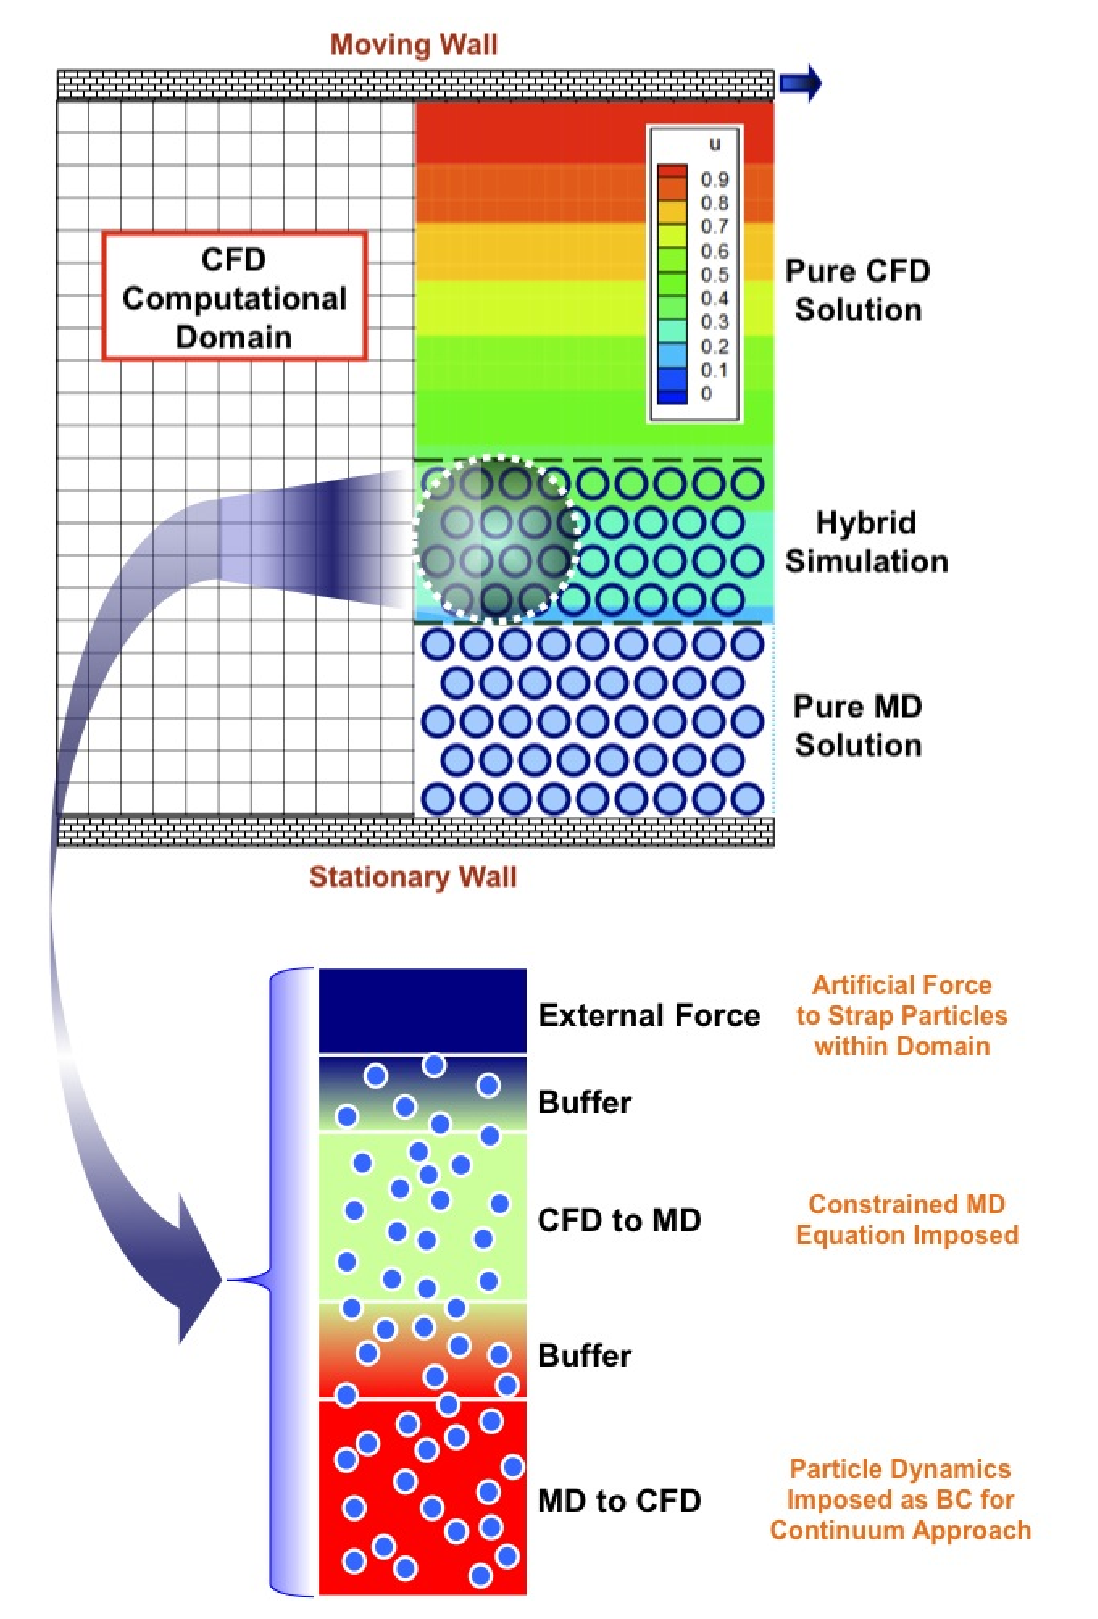
\includegraphics[scale=0.45]{fig1.eps}
\caption{\small Schematic of CFD/MD Coupled Simulation of Channel Flow}
\label{Fig:Couette}
\end{figure}
%%%%% FIGURE %%%%%

In this study, we used the MPI version of the in-house incompressible CFD code~\cite{Lee} for CFD and the MPI version of the in-house modified version of LAMMPS~\cite{LAMMPS} for MD.  As illustrated in Fig.~\ref{Fig:Couette}, the coupling mechanism is the key component for successful hybrid CFD/MD simulations and our implementation follows the literature~\cite{Nie},~\cite{Yen} . In brief, the hybrid region where the coupling mechanism between MD region and CFD region is executed comprises five sub-regions.  In the CFD boundary grid region positioned near the pure MD region, velocities of particles obtained with MD are averaged and used for boundary condition for the corresponding CFD computational cells.  The MD boundary zone is placed above the CFD boundary zone and here, information on velocities from the CFD grid are imposed on particles in the zone through dynamically constrained equation of motion for MD.  Between these zones, a buffer layer exists to avoid any harmful direct influences from one zone to another zone.  The truncated and shifted Lennard-Jones potential is used for interactions of particles in MD simulation.

As clearly indicated in Fig.~\ref{Fig:Couette}, the most prominent computational challenge is how to run efficiently two separate stand alone applications that require frequent information exchange.  In other words, the time-to-solution heavily relies on how to avoid waiting situations in particular for information exchange steps.  In that sense, our SAGA-based framework is capable of build one efficient runtime environment for this kind of coupled simulations.  Here, note that imbalance arising from different performance between two distinguishably heterogeneous applications, CFD and MD, causes an unavoidable time gap for the arrival time to the exchange step, which is only curable with dynamical resource allocation implemented with a load-balancing mechanism.   



%\Nkimnote{ }
%-------------------------------------------------------------------------
\section{SAGA and SAGA-based Frameworks for Large-Scale and Distributed Computation}

The Simple API for Grid Applications (SAGA) is an API standardization effort within the Open Grid Forum (OGF)~\cite{ogf_web}, an international standards development body concerned primarily with standards for distributed computing.  SAGA provides a simple, POSIX-style API to the most common Grid functions at a sufficiently high-level of abstraction so as to be %able to be
independent of the diverse and dynamic Grid environments. The SAGA specification defines interfaces for the most common Grid-programming functions grouped as a set of functional packages (Fig.~\ref{Fig:SAGA1}). Some key packages are:

\begin{figure}[!ht]
 \begin{center}
     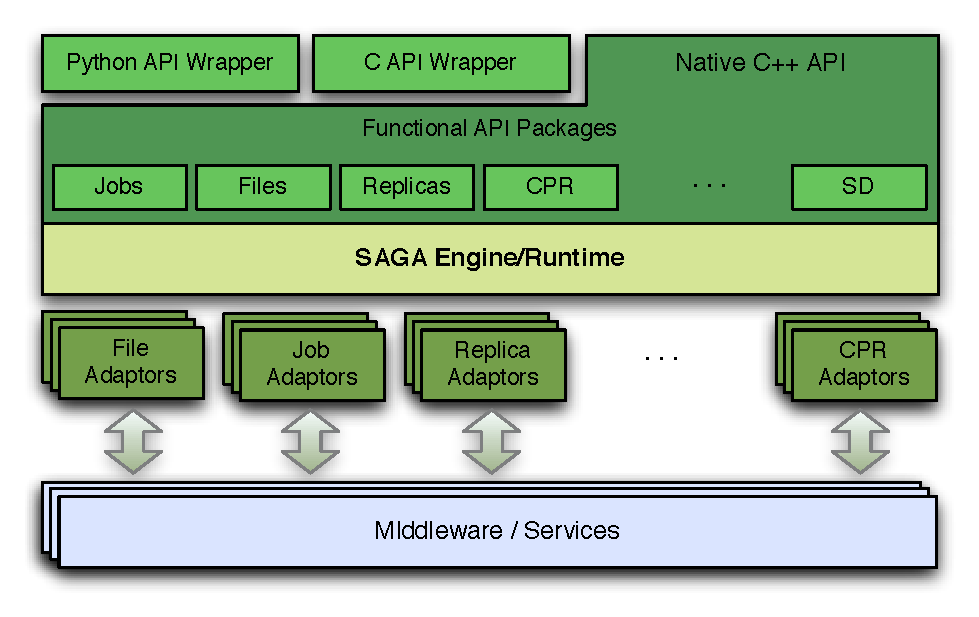
\includegraphics[width=0.40\textwidth]{stci_saga_figures-1.pdf}
 \end{center}
\caption{\small Layered schematic of the different components
  of the SAGA landscape. At the topmost level is the simple integrated API which provides the basic functionality for distributed computing. Our BigJob abstraction was built upon this SAGA layer using Python API wrapper} \label{sagalayer}
\end{figure}

%\begin{itemize}\addtolength{\itemsep}{-0.8\baselineskip}


\begin{itemize}
\item File package - provides methods for accessing local and remote
 filesystems, browsing directories, moving, copying, and deleting
 files, setting access permissions, as well as zero-copy reading and
 writing
\item Job package - provides methods for describing, submitting,
 monitoring, and controlling local and remote jobs. Many parts of
 this package were derived from the largely adopted
 DRMAA % ~\cite{drmaa_url}
 specification.
\item Stream package - provides methods for authenticated local and
 remote socket connections with hooks to support authorization and
 encryption schemes.
\item Other Packages, such as the RPC (remote procedure call) and Replica
 package
\end{itemize}


%\skonote{Introduction of PilotJob and BigJob (1 or 2 paragraphs) : What is PilotJob, BigJob / what have been done so far and how effective it was when using BigJob}



%\skonote{Joohyun, can you check this paragraph and improve it? In this paragraph, I was going to talk about 'Structure and Simulation Flow of BigJob Abstraction for Coupled Simulation'.}


Fig.~\ref{Fig:BigJob_Structure} shows the structure of BigJob and its operation flow. When a BigJob is submitted to the remote resource, the application manager monitors the status of this pilot-job through the advert service. When resources are allocated to the BigJob, the application manager divides obtained resources to its sub-jobs and a coupled simulation starts under the control of a multi-physics agent in the remote resource. Advert service keeps on getting the status of a pilot-job from the queuing system and the status of sub-jobs from multi-physics agent, also delivering these information to the application manager by a push-pull mechanism. The application manager watches the status of sub-jobs and decides the next event when the coupled simulation is finished. When one default BigJob is launched, subtasks keeps running until final solution is achieved and the manager quits the pilot-job at that time. In cases multiple BigJobs are submitted for the same simulation or a load balancing function is included, sub-jobs experience several restarts from their checkpointing data, reflecting changed processor allocation to each application. In former case, resource allocation to each sub-job follows a pre-defined map according to the number of BigJobs allotted to this simulation: In latter case, resource allocation to each sub-job becomes dynamic according to its performance, to be discussed in the next section.

%%%%% FIGURE %%%%%
\begin{figure}
\centering
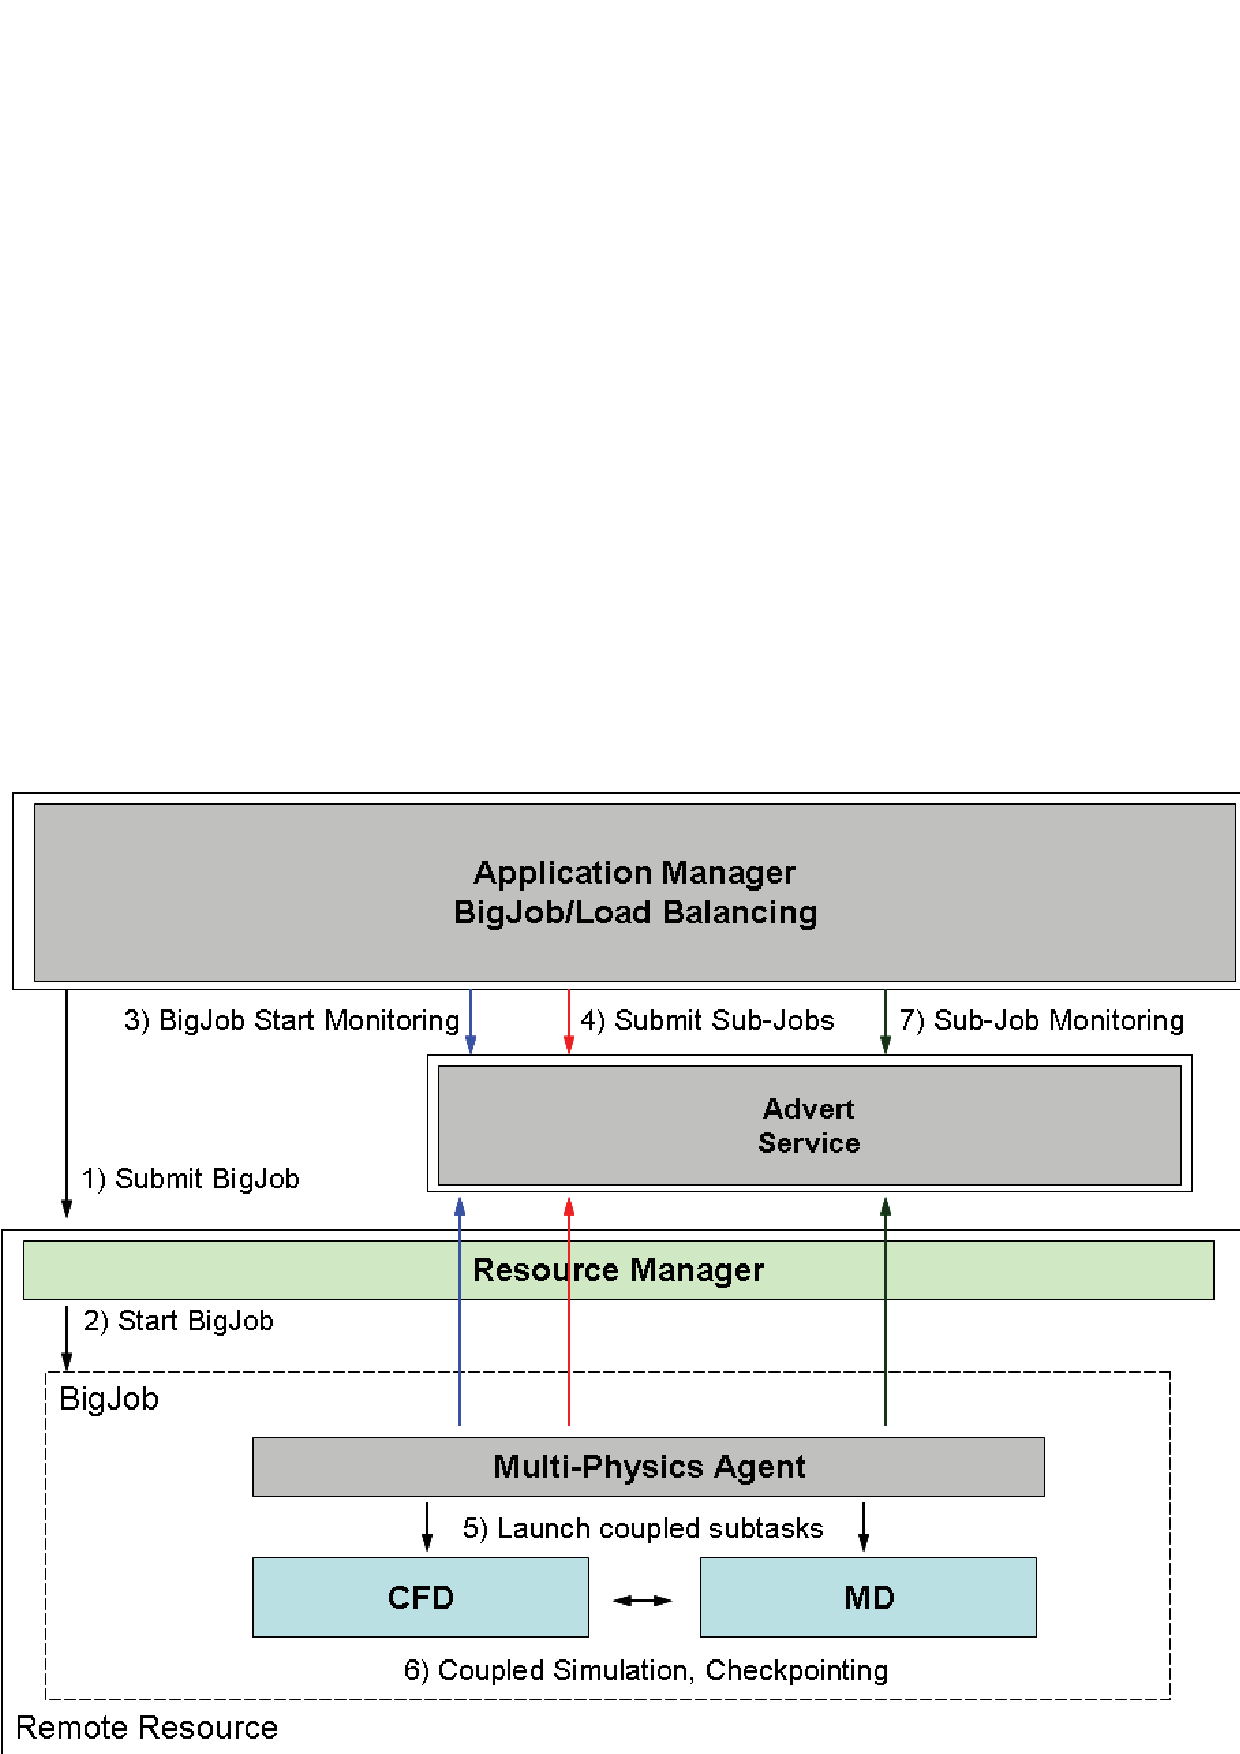
\includegraphics[scale=0.38]{Structure_of_BigJob}
\caption{\small Architecture of the Controller/Manager and Control Flow: Application manager is responsible for job management including BigJob and sub-job submission, their status monitoring functions. We implement a load balancing module, and migration service based on job information. Application agent system resides on each HPC resource and conducts job information gathering as well as communication with application manager via the advert service}
\label{Fig:BigJob_Structure}
\end{figure}
%%%%% FIGURE %%%%%



%-------------------------------------------------------------------------
\section{Load Balancing for Coupled Multi-Physics Simulation}


SAGA and its pilot-job framework (BigJob) enable coupled, yet distinct simulations to be
% by resolving the concurrency problem when coupled application codes are individually
submitted to queuing system.  This is done by submitting one container job, and re-distributing its processors to each task.  Also, total execution time can further be reduced by assigning more BigJobs and dynamically reallocating resources to each sub-task with increased number of processors.
However, the flexibility to re-distribute resources (processors) to the individual task, does
not imply efficient utilization. This is the responsibility of a load-balancer (LB)
We will discuss the implementation and algorithm of this LB; it is important
to mention that the LB functions in the context of the SAGA-BigJob framework.
% As the current simulation requires frequent data exchange between CFD and MD during the simulation, it is likely to increase communication cost (strictly, waiting time for communication in one application) if their loads are not well balanced, which is quite different from former BigJob application~\cite{Jha:2009} where data exchange takes place when sub-tasks stopped temporarily.

% Meanwhile, checking sub-tasks' performances and controlling their operation for load balancing runs counter to SAGA's philosophy of "using services without changing the application source". Thus, help from application side is necessary to employ a load balancing function on a BigJob.

Each applications load is determined by its elapsed time to run the evolution loop. Here, time for initialization or inter-domain data exchange are excluded from the counting, because they are one-time event or irrelevant to application's performance. As the result of load balancing is reflected in the next launch of simulation codes, applications should be able to restart from their checkpointing data. Also, they should be equipped with generalized domain partitioning routine to run simulation with any number of processors, without harming their parallel efficiency a lot.  If above conditions are satisfied, BigJob application manager,
can be interfaced with the LB to implement the dynamic resource allocation between tasks.
% load balancing between subtasks before applications restart from the previous state.
The idea of current load balancing algorithm is to assign more processors to a sub-task with more runtime until two codes show the same runtime. We have adopted some assumptions to simplify load balancing procedure and apply the algorithm without considering applications' characteristics and individual code's scalability. Assumptions are, (1) Each application code follows the ideal parallel efficiency.
(2) All processors in one node is assigned to one sub-job.

%\begin{tabular}{|l|}
%\hline

%Let computation time of two applications by $t_CFD$ and $t_MD$, processors to each domain by $PE_CFD$ and $PE_MD$, respectively.
%Total workload $W_TOT$ is going to be \\

%\begin{equation}
%\begin{center}
%W_{TOT} = W_{CFD} + W_{MD} = PE_{CFD} \ times t_{CFD} + PE_{MD} \ times t_{MD}
%= PE_{TOT} \times t_{TOT}
%\end{center}
%\end{equation}

Let the computation time of two applications as $t_{CFD}$ and $t_{MD}$, processors to each domain as $PE_{CFD}$ and $PE_{MD}$, respectively. Based on assumption (1), workload on each application remains the same after the reallocation of resources,
\begin{eqnarray}
%\begin{center}
W_{CFD} &=& PE_{CFD} \times t_{CFD} = PE_{CFD}' \times t_{CFD}', \nonumber \\
W_{MD} &=& PE_{MD} \times t_{MD} = PE_{MD}' \times t_{MD}'
%$t_{CFD} = \frac {PE_{CFD} \times t_{CFD}} {PE_{CFD}} , ~~ t_{MD} = \frac {PE_{MD} \times t_{MD}} {PE_{MD}}$
%\end{center}
\label{eq:SimTime_EachTask}
\end{eqnarray}
Still, total number of processor remains the same:
\begin{equation}
%\begin{center}
PE_{TOT} = PE_{CFD} + PE_{MD} = PE_{CFD}' + PE_{MD}'
%\end{center}
\label{eq:PECondition}
\end{equation}
Our objective is to reduce the computation time of an over-loaded subtask until two simulations show the same computation time, $t_{CFD}' = t_{MD}'$. Then, Equation~\ref{eq:SimTime_EachTask} and Equation~\ref{eq:PECondition} concludes the optimal processors for one subtask would be
\begin{eqnarray}
%\begin{center}
PE_{CFD}' & = & \frac {W_{CFD}} {(W_{CFD} + W_{MD})} \times PE_{TOT}
%\end{center}
\end{eqnarray}
The other sub-job will follow the similar expression.
The optimal processor distribution from above equation will return a float value. Also, considering the second assumption, which is the policy of many supercomputing center, the above distribution needs to be asymptotic. If CPU cores in one node is $N_{UNIT}$,
%$N_{UNIT} \times S < PE_{CFD}' < N_{UNIT} \times (S+1)$, we can choose the optimal condition by comparing $MAX(t_{CFD}',t_{MD}')$ between upper and lower bound of processor allocation.
optimal condition can be gained by finding $S = int(PE_{CFD}' / N_{UNIT})$ and comparing $MAX(t_{CFD}',t_{MD}')$ in cases CFD task is allocated with $N_{UNIT} \times S$ or $N_{UNIT} \times (S+1)$.


%\hline
%\end{tabular}

%The control-flow within the BigJob Application-Manager when supporting a LB modules is shown in Fig.~\ref{Fig:BigJob_LB}. When one simulation loop is finished, the performance data of each subtask is sent to the load balancing module and it computes optimal resource distribution. Sub-job launcher restarts coupled application codes from their checkpointing data, according to the result of load balancing function. This process iterates until coupled simulation finalizes and processor allocation moves to the optimal condition during this process.

%%%%% FIGURE %%%%%
%\begin{figure}
%\centering
%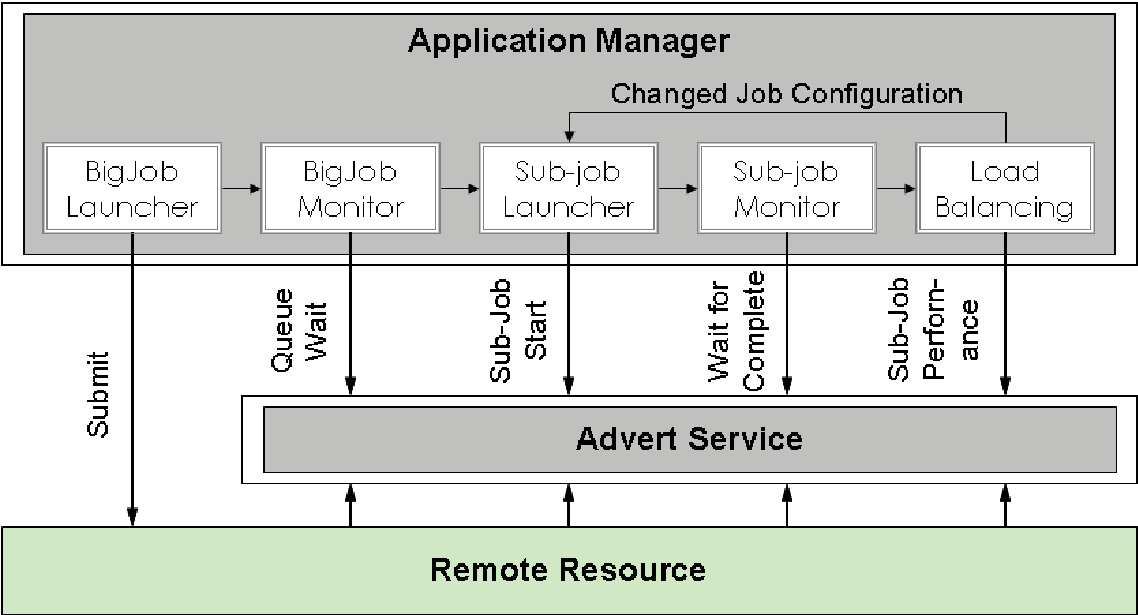
\includegraphics[scale=0.40]{BigJob_with_Load_Balance}
%\caption{\small Operation Flow of a BigJob with Load Balancing Function}
%\label{Fig:BigJob_LB}
%\end{figure}
%%%%% FIGURE %%%%%



%-------------------------------------------------------------------------
\section{Dynamic Resource Allocation for Coupled Simulations: Three Scenarios }

In Section 2, we have argued the challenges of running a coupled multi-physical simulation on a conventional queuing system as (i) Hardness to start multiple applications concurrently; (ii) Inability to balance the load among domains, and (iii) Fixed number of allocated resources throughout the simulation.  To resolve the co-scheduling and load-imbalance issues, and with the ultimate aim of reducing the time to solution, we have used the BigJob abstraction with load balancing module to the coupled simulation. % With the ultimate aim of reducing the total simulation time, we investigate acquiring idle resources during the simulation, by launching multiple BigJobs for one coupled simulation.
Three different real scenarios arise. In the first, a single BigJob is utilized to run the coupled-simulations, first without, and then with the LB redistributing resources based upon their individual performance. One component maybe relieved of its resources for the greater good. In the second Use Case, In the second case, two BigJobs are started together, but often one BigJob starts before the other; to increase efficiency both coupled simulations start with whatever resources are available as part of the first (to run) BigJob. When the other BigJob becomes active, there is a dynamic redistribution of tasks, such that
the larger of the two simulations is assigned the bigger BigJob. The variant of the above when
the two BigJobs are on different machines forms Use Case 3. In the remainder of this section we discuss
the details of these three different Use Cases.

% We compare the performance as measured by TTS using the benchmark case to be the situation when we do not have the ability to utilize the BigJob concept and thus each simulation interacts with the queueing system differently, and thereby each must be in an Active state before both can start running.

%\jhanote{please be sure to use co-scheduling where appropriate and not concurrency}

\subsection{One BigJob with Load Balancing}
Fig.~\ref{Fig:OneBJ_Flow} shows the flow of a coupled simulation with the conventional job submission and through one BigJob. In a conventional way, individual tasks with resource requirements of $PE_{CFD}$ and $PE_{MD}$, respectively, are independently submitted to the conventional queuing system and job scheduler recognizes these coupled tasks as two distinct jobs. Thus, they are going to start at a different time, except when enough resources are available. In this case, both tasks wait on the queue when no job is allocated, the first allocated job idles to do data exchange with its counterpart, and run actual simulation after both jobs are allocated. On the other hand, in a BigJob simulation, a pilot job with the size of $PE_{CFD}+PE_{MD}$ is submitted to the queue and coupled simulation directly starts when the resource is assigned on this BigJob. By using a BigJob, a user can save his/her account consumption on inactive mode in conventional job submission, while total runtime is the same if the resource distribution to sub-jobs is identical. However, eliminating inactive mode does not guarantee total simulation time is reduced, because waiting to get one bigger allocation may happen to take more than getting two allocations with smaller chunks. The same situation can happen to the load-balanced case with one BigJob, which satisfies the reduction of total runtime compared to other examples.

%%%%% FIGURE %%%%%
\begin{figure}
\centering
\includegraphics[scale=0.40]{Simulation_Time_of_One_BigJob.eps}
\caption{\small Comparison of dependencies encountered for coupled-simulations submitted as conventional Jobs, to the scenario when using Pilot-Jobs (BigJob). Here we use only 1 BigJob. The conventional mode of submission experiences three phases of queue waiting (all jobs are waiting: $t_1-t_0$), inactive mode (one job is waiting for another: $t_2-t_1$), and active running (running a coupled simulation: $t_f-t_2$). On the other hand, inactive mode disappears when coupled simulation runs within one BigJob, as an allocated BigJob distributes its resource to sub-jobs.}
\label{Fig:OneBJ_Flow}
\end{figure}
%%%%% FIGURE %%%%%


Table ~\ref{table:oneBJ_Test} shows elapsed time on running above test cases: conventional job submission, one default BigJob launch and one BigJob with load balancing. These tests were conducted on supercomputing resources in LONI (Louisiana Optical Network Initiative)~\cite{LONI_web} and tested resources of eric, oliver and louie have the same specification with 4 processors in each node. A coupled simulation has been conducted by using 32 processors with two different processor allocations to subtasks. Application codes experience four restarting from their checkpointing data in load balancing test, while simulation keeps running until it completes in baseline and default BigJob tests.
When the same number of processors are allocated to CFD and MD tasks, one BigJob simulation with LB shows better performance on runtime compared to other two cases. Load balancing function changes the resource distribution to the best condition after the first simulation loop and 8 processors from CFD task are moved to MD simulation from the next start. As a result, total runtime is saved by about 20 percent compared to other test cases. On the other hand, a load-balanced BigJob shows worse performance in the latter test when initial processor distribution is an optimal condition, because running a load balancing function and trying checkpointing and restarting subtasks becomes additional costs. Comparing results between conventional job allocation and one BigJob simulation (with or without LB), it is guaranteed that a lot of computational cost on idling is saved. However, it does not guarantee that one BigJob allocation satisfies the reduction of total simulation time: waiting time on the queue purely depends on the condition of remote resource.


% Elapsement for a CFD/MD Coupled Simulation by using Conventional Queueing System and a BigJob Abstraction. Above table shows total simulation time when 8 processors are allocated to CFD and 24 processors on MD task, which is initially well-balanced allocation: below one represents another test with 16 processors allocated to each task, an imbalanced simulation. Values in table shows averaged time in seconds, values within a parenthesis are standard deviation of time elapsed; the average is taken over 5 distinct
% experiments. \newline }

\setlength{\tabcolsep}{1pt}
\begin{table}[!ht]
\begin{center}

\caption{\small Results for performance data using BigJob with and without LB. The Baseline Simulation represents the case when BigJob is not used; in this case, the time to start is dominated by the Inactive Mode of the longer waiting task. The use of BigJob resolves, this as can be seen by the reduced inactive mode time in columns 3 and 4. The starting configuration assigns resources equally between CFD-MD -- 16px each. However, after a few iterations of the LB the configuration is 8-24. It is with this configuration that the performance is better with LB, than without the LB 1370 $\pm 98$ vs 1641 $\pm$ 162. The starting configuration of the second set (8-24) is a ``balanced configuration'' which is why there is no performance gains on using the LB. Values in table shows averaged time in seconds, values within a parenthesis are standard deviation of time elapsed; the average is taken over 5 distinct experiments}
% experiments. }
%\label{table:systems}
\label{table:oneBJ_Test}
\begin{tabular}{ c|| c | c | c }
\hline
16-16 & Baseline Simulation & BigJob (no LB) & BigJob (LB) \\
\hline
\hline
Waiting on & 3000     & 10834  & 15201  \\
the Queue  & (4136)   & (4593) & (10968) \\
\hline
Inactive   & 10300    & 4      & 4  \\
Mode       & (15327)  & (0)    & (0) \\
\hline
Active     & 1672     & 1641   & 1370 \\
Runtime    & (246)    & (162)  & (98) \\
\hline
Total      & 14973    & 12480  & 16577 \\
Time       & (19213)  & (4430) & (11004) \\
\hline
\end{tabular}
\begin{tabular}{ c|| c | c | c }
\hline
8-24 & Baseline Simulation & BigJob (no LB) & BigJob (LB) \\
\hline
\hline
Waiting on & 1900 & 3372 & 10344  \\
the Queue & (1873) & (6450) & (6767) \\
\hline
Inactive & 5486 & 4 & 4 \\
Mode & (10318) & (0) & (0) \\
\hline
Active & 1171 & 1169 & 1280 \\
Runtime & (175) & (72) & (81) \\
\hline
Total & 8557 & 4545 & 11629 \\
Time & (11882) & (6457) & (6720) \\
\hline
\end{tabular}
\end{center}
\end{table}


A number of experiments have been conducted to validate the performance of a load balancing function with different BigJob size. Fig.~\ref{fig:LB_Graph} shows the change of processor allocation to sub-jobs and their runtime at every start. A BigJob with 24 processors is tested with two kinds of initial processor distribution between CFD and MD, 8 to 16 or 16 to 8. In all simulations, the load balancing function detects the ratio of 4 and 20 between CFD and MD tasks are optimal and converges to this ratio at the next restart, except one case when CFD solution experiences unexpected overload initially. Even in this case, load balancing function traces the optimal load allocation during the iteration and this demonstrates the stability of current load balancing function. After the balancing, runtimes of CFD and MD jobs become very close, 219 seconds for CFD and 236 for MD task.

%%%%% FIGURE %%%%%
\begin{figure}
\centering
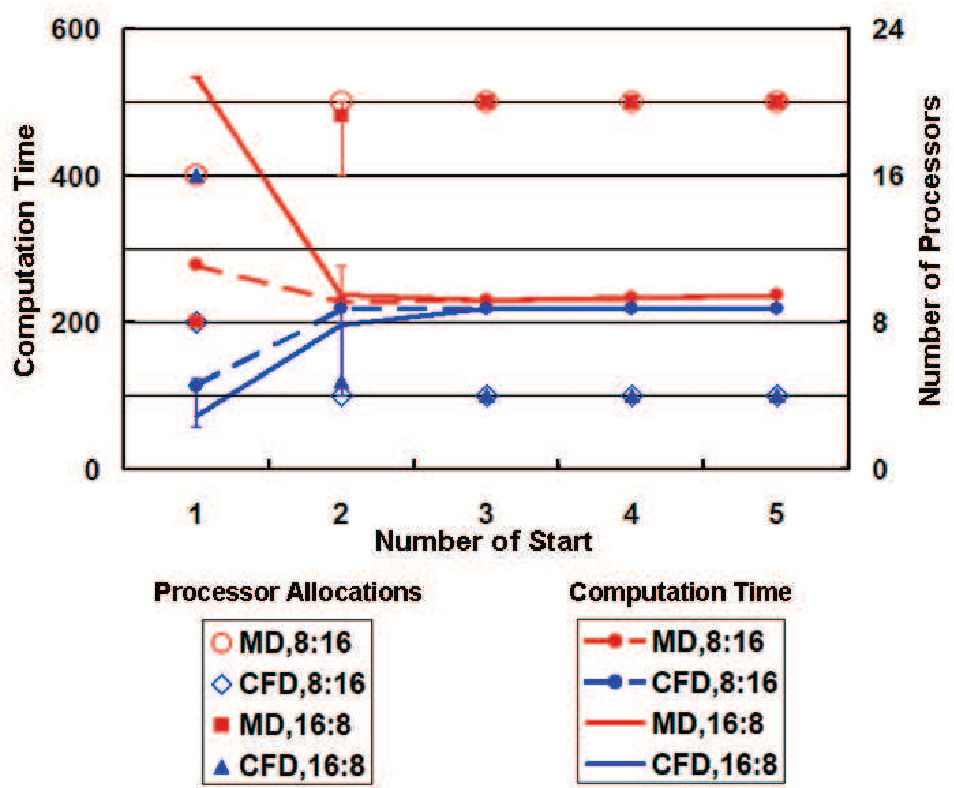
\includegraphics[scale=0.45]{LB_Graph2}
\caption{\small Convergence of a Load Balancing Function and Runtime of Sub-jobs. Lines show runtime change of each sub-job, symbols represent the history of load balancing at every start/restart. In all cases when initial processor distribution between CFD and MD tasks are 8 to 16 or 16 to 8, load balancer leads the processor allocation to 4 and 20 and coupled simulation time reduces to be around 235 seconds. All tests were conducted 5 times; the bars in the graph represent minimum and maximum values from the 5 tests. \jhanote{let us discuss this at 3pm}}
\label{fig:LB_Graph}
\end{figure}
%%%%% FIGURE %%%%%


Though the above results show the large performance gain by employing a load balancing algorithm, some limitations are also observed. First, as the function only refers to the computation cost at given processor distribution and moves to the optimal condition iteratively, it takes time to achieve a converged resource allocation if initial processor allocation starts from other extreme. Second and furthermore, the algorithm itself should be refined to distinguish the computational cost from inter-processor communication within one application code and control both factors. Also, the load balancing module needs to be expanded to cover multiple BigJob allocations for one coupled simulation, when running a subtask across BigJobs becomes possible.


\subsection{Two BigJobs from a Single Site or Multiple Sites}


As illustrated in Figure~\ref{Fig:TwoBigJobs}, runtime environment for coupled multi-physics simulations would benefit from dynamic resource availability exploited by BigJob implementation. In brief, it is possible to assign more CPUs for a slowing application when another BigJob becomes available. Compared with one BigJob allocation for a coupled simulation in Figure~\ref{Fig:OneBJ_Flow}, two smaller BigJob submissions with sizes of CFD and MD will enable faster start of coupled subtasks. Also, when next BigJob is also allocated to this coupled simulation, total job size will be the same as one BigJob submission. In a word, resource allocation and simulation flow is identical to the conventional job submission, but inactive idling in a conventional case disappears as a BigJob framework starts coupled subtasks with smaller number of processors when first job is allocated. So, submitting two BigJobs guarantees the reduction of total simulation time compared to conventional job submission, if all conditions are identical. If this two BigJob submission is applied on multiple sites, it is more likely to get two allocations faster than requesting two jobs in the same site. However, faster launch of two BigJobs does not guaranteed save of total simulation time, because time for data exchange between applications will also increase if distributed resources cooperate.


%%%%% FIGURE %%%%%
\begin{figure} \centering \includegraphics[scale=0.40]{Simulation_Time_of_Two_BigJobs.eps} \caption{\small Schematic comparing the distribution of simulations when 2 BigJobs are used, first on the same physical machine, then on different (distributed) machines. In both cases, coupled sub-jobs start running when the first BigJob is allocated at $t=t_1$ and experience resource reallocation with increased amount when the next BigJob becomes available. When two BigJobs are allocated, each sub-job occupies one BigJob and data exchange between jobs takes place across BigJobs.}  \label{Fig:TwoBigJobs} \end{figure}
%%%%% FIGURE %%%%%


In Table~\ref{table:TwoBigJobs}, test measurements for performance gains are summarized. The scenario for this testing is simple for clarifying benefits.  Initially, two BigJobs are submitted to one HPC resource or two HPC resources.  Once the first bigjob becomes available, two applications are submitted as two subtasks with pre-defined cpus to the bigjob, and then when another bigjob becomes available later, two subtasks for each application is reconfigured by assigning the entire cpus of a bigjob to one application.  Table  ~\ref{table:TwoBigJobs} shows performance gains with such a scenario in terms of MD run time.  In this simple scenario, other complicated aspects such as file transfer, in particular between two distributed resources are not considered but in the future study, the overall performance will be optimized by considering them.

% Performance gains with two bigjobs. Performance is measured with CPU times consumed by MD, since test cases we used always require longer cpu times for MD than those of CFD.  Performance gains with additionally available bigjob can be seen by comparing MD CPU times with those obtained with the initial bigjob.  Measurements were carried out with LONI cluster systems.  louie and poseidon are dell cluster systems having 128 nodes with 4 cores in a node. \jhanote{add bigjob size --- which 8 and 16} Test 1 and 2 correspond to Use Case 2; Test 3 and 4 correspond to Use Case 3 \newline }

\begin{table}[!h]
\begin{center}
 \caption{\small
Performance measures for Use Cases 2 and 3. We take the time of the MD simulation as a measure of performance.
For Test 1 and 2, we compare the time taken (for the MD simulation) before and after the availability of
the second BigJob. As can be seen, the time to solution is significantly lower. This is now because
the entire second BigJob is available to the MD simulation.
For Test 3 and 4, the second BigJob (i.e the one to start later) is launched on a different machine
from the first BigJob. For similar reasons to Test 1\&2, the time to solution is lower when the
second BigJob starts. This situation will win over the single BigJob scenario, despite of transfer/set-up times. For Test 1-3, the size of the first BigJob is 8px, whilst the size of the second (later available) BigJob is 16px. For Test the first BigJob is 16px and the second BigJob is 32px.}
\label{table:TwoBigJobs}
\begin{tabular}{ c| c c c c }
\hline
& Test 1   & Test 2 & Test 3   & Test 4 \\
\hline
number of sites & 1 & 1 & 2 & 2  \\
site names & P & L  & L + P & L + P \\
\hline
(one bigjob available) & & & & \\
number of cpus assigned & 4 & 4 & 4 & 8 \\
MD CPU time  (sec) & 1037.2 & 1045.2 & 1049.0 & 534.2  \\
\hline
(two BigJobs available) & & & & \\
number of cpus assigned & 16 & 16 & 16 & 32 \\

MD CPU time  (sec) & 277.21 & 277.63  & 276.8 & 150.4  \\

\hline
\end{tabular}
\end{center}
\end{table}


In summary, use of a BigJob will eliminate idling operation of a subtask, which waits for another application to start running. Also, employing a load balancing function will let coupled codes use allocated resources more efficiently. Furthermore, using two BigJobs promotes the reduction of total simulation time, compared to conventional job submission. Meanwhile, launch of two BigJobs does not intend to use resources more efficiently than conventional job allocation, but intend to save total simulation time more than one BigJob test case, by utilizing more available resources. Remember that having multiple BigJob allocations is to increase the computing power for a specific simulation, not to use optimally within given circumstances.


%-------------------------------------------------------------------------
\section{BigJob: A General Purpose Pilot-Job}

We are able to submit a SAGA-based Pilot-Job to Condor in addition to TeraGrid resources -- to both a Condor-G interface and a Condor resource pool. To that end we use Condor's native pilot-job (Glide-In) for Condor resources, through the SAGA Condor adaptor. This allows us to concurrently make use of high performance resources on the TeraGrid and high-throughput resources such as the Condor pools at Purdue and LONI. Having the capability to run pilot jobs on both types of resources through a unifed abstract interface with varying underlying mechanisms presents new vistas for infrastructure interoperabiltiy, such as the TeraGrid and the Open Science Grid.

To demonstrate that a single SAGA-based BigJob interface works for both, we started a BigJob on Queen Bee (shared TeraGrid LONI machine), to which we submitted a MD simulation. Once the MD simulation started, the coupled CFD simulation is submitted to the Condor Pool at Purdue through the Condor Glide-In. The total time spent running on QueenBee was 5328 seconds, and the total run time on the Condor poll was 1015 seconds for a reduced number of iterations. The reduction in problem size was necessary due to the lack of a working MPI Condor universe on an accessible resource.

\section{Conclusions}
Increasing accessibility to High Performance Computing and advances in software development utilizing parallelisms implemented in different granularity are, perhaps, two critical components for recent numerous successful outcomes with large scale scientific calculations in various domains. Nonetheless, it is not trivial to integrate a targeted scientific application with a resource management system that is aware of the challenges arising from the distributed computing as well as the local scheduler implemented with the local resource management policy.  
In this work, we report our development for efficient runtime environment targeting the coupled multi-physics application comprising MD and CFD as two coupled standalone applications.  Overcoming the co-scheduling requirements and implementing dynamic resource allocation mechanism were two main goals motivating a novel development and our test runs demonstrated its potential for large scale scientific simulations benefiting scientific problems that are only tackled by a coupled hybrid MD-CFD calculation.
Our development is built upon the BigJob framework enabled by the SAGA.  The cycle of the development for core BigJob management system is significantly helped by using the SAGA with which the simple and consistent interface for managing HPC resources is easily achieved resulting the agile and flexible development.
We tested our development for three cases and demonstrated its capability.  In addition, the use cases includes the usage of the Condor-glide-in as our BigJob framework is closely related.  In spite of simple nature of our test problems, already our development showed many promises for a successful large scale simulation.  Some of those are i) employment of load balancing mechanism ii) advantages from implementation of dynamic allocation in heterogeneous distributed computing resources iii) simple solution for the co-scheduling requirements for the coupled tasks.
% Please direct any questions to the production editor in charge of these
% proceedings at the IEEE Computer Society Press: Phone (714) 821-8380, or
% Fax (714) 761-1784.

\section*{Acknowledgment}
This work is part of the Cybertools (http://cybertools .loni.org) project and primarily funded by NSF/LEQSF (2007-10)-CyberRII-01. Important funding for SAGA has been provided by the UK EPSRC grant number GR/D0766171/1 (via OMII-UK).  This work has also been made possible thanks to computer resources provided by LONI.  We thank Andre Luckow for initial work on BigJob, Lukasz Lacinski for help with SAGA deployment (via HPCOPS NSF-OCI 0710874) and Joao Abecasis for his work on the SAGA Condor adaptors.

%-------------------------------------------------------------------------
\nocite{ex1,ex2}
%\bibliographystyle{latex8}
\bibliographystyle{IEEEtran}
\bibliography{saga_tg08}


\end{document}




%-------------------------------------------------------------------------
\section{Instructions}

Please read the following carefully.

%-------------------------------------------------------------------------
\subsection{Language}

All manuscripts must be in English.

%-------------------------------------------------------------------------
\subsection{Printing your paper}

Print your properly formatted text on high-quality, $8.5times 11$-inch
white printer paper. A4 paper is also acceptable, but please leave the
extra 0.5 inch (1.27 cm) at the BOTTOM of the page.

%-------------------------------------------------------------------------
\subsection{Margins and page numbering}

All printed material, including text, illustrations, and charts, must be
kept within a print area 6-7/8 inches (17.5 cm) wide by 8-7/8 inches
(22.54 cm) high. Do not write or print anything outside the print area.
Number your pages lightly, in pencil, on the upper right-hand corners of
the BACKS of the pages (for example, 1/10, 2/10, or 1 of 10, 2 of 10, and
so forth). Please do not write on the fronts of the pages, nor on the
lower halves of the backs of the pages.


%------------------------------------------------------------------------
\subsection{Formatting your paper}

All text must be in a two-column format. The total allowable width of
the text area is 6-7/8 inches (17.5 cm) wide by 8-7/8 inches (22.54 cm)
high. Columns are to be 3-1/4 inches (8.25 cm) wide, with a 5/16 inch
(0.8 cm) space between them. The main title (on the first page) should
begin 1.0 inch (2.54 cm) from the top edge of the page. The second and
following pages should begin 1.0 inch (2.54 cm) from the top edge. On
all pages, the bottom margin should be 1-1/8 inches (2.86 cm) from the
bottom edge of the page for $8.5 \times 11$-inch paper; for A4 paper,
approximately 1-5/8 inches (4.13 cm) from the bottom edge of the page.

%-------------------------------------------------------------------------
\subsection{Type-style and fonts}

Wherever Times is specified, Times Roman may also be used. If neither is
available on your word processor, please use the font closest in
appearance to Times that you have access to.

MAIN TITLE. Center the title 1-3/8 inches (3.49 cm) from the top edge of
the first page. The title should be in Times 14-point, boldface type.
Capitalize the first letter of nouns, pronouns, verbs, adjectives, and
adverbs; do not capitalize articles, coordinate conjunctions, or
prepositions (unless the title begins with such a word). Leave two blank
lines after the title.

AUTHOR NAME(s) and AFFILIATION(s) are to be centered beneath the title
and printed in Times 12-point, non-boldface type. This information is to
be followed by two blank lines.

The ABSTRACT and MAIN TEXT are to be in a two-column format.

MAIN TEXT. Type main text in 10-point Times, single-spaced. Do NOT use
double-spacing. All paragraphs should be indented 1 pica (approx. 1/6
inch or 0.422 cm). Make sure your text is fully justified---that is,
flush left and flush right. Please do not place any additional blank
lines between paragraphs. Figure and table captions should be 10-point
Helvetica boldface type as in
\begin{figure}[h]
  \caption{Example of caption.}
\end{figure}

\noindent Long captions should be set as in
\begin{figure}[h]
  \caption{Example of long caption requiring more than one line. It is
    not typed centered but aligned on both sides and indented with an
    additional margin on both sides of 1~pica.}
\end{figure}

\noindent Callouts should be 9-point Helvetica, non-boldface type.
Initially capitalize only the first word of section titles and first-,
second-, and third-order headings.

FIRST-ORDER HEADINGS. (For example, {\large \bf 1. Introduction})
should be Times 12-point boldface, initially capitalized, flush left,
with one blank line before, and one blank line after.

SECOND-ORDER HEADINGS. (For example, {\elvbf 1.1. Database elements})
should be Times 11-point boldface, initially capitalized, flush left,
with one blank line before, and one after. If you require a third-order
heading (we discourage it), use 10-point Times, boldface, initially
capitalized, flush left, preceded by one blank line, followed by a period
and your text on the same line.

%-------------------------------------------------------------------------
\subsection{Footnotes}

Please use footnotes sparingly%
\footnote
  {%
    Or, better still, try to avoid footnotes altogether.  To help your
    readers, avoid using footnotes altogether and include necessary
    peripheral observations in the text (within parentheses, if you
    prefer, as in this sentence).
  }
and place them at the bottom of the column on the page on which they are
referenced. Use Times 8-point type, single-spaced.


%-------------------------------------------------------------------------
\subsection{References}

List and number all bibliographical references in 9-point Times,
single-spaced, at the end of your paper. When referenced in the text,
enclose the citation number in square brackets, for example~\cite{ex1}.
Where appropriate, include the name(s) of editors of referenced books.

%-------------------------------------------------------------------------
\subsection{Illustrations, graphs, and photographs}

All graphics should be centered. Your artwork must be in place in the
article (preferably printed as part of the text rather than pasted up).
If you are using photographs and are able to have halftones made at a
print shop, use a 100- or 110-line screen. If you must use plain photos,
they must be pasted onto your manuscript. Use rubber cement to affix the
images in place. Black and white, clear, glossy-finish photos are
preferable to color. Supply the best quality photographs and
illustrations possible. Penciled lines and very fine lines do not
reproduce well. Remember, the quality of the book cannot be better than
the originals provided. Do NOT use tape on your pages!

%-------------------------------------------------------------------------
\subsection{Color}

The use of color on interior pages (that is, pages other
than the cover) is prohibitively expensive. We publish interior pages in
color only when it is specifically requested and budgeted for by the
conference organizers. DO NOT SUBMIT COLOR IMAGES IN YOUR
PAPERS UNLESS SPECIFICALLY INSTRUCTED TO DO SO.

%-------------------------------------------------------------------------
\subsection{Symbols}

If your word processor or typewriter cannot produce Greek letters,
mathematical symbols, or other graphical elements, please use
pressure-sensitive (self-adhesive) rub-on symbols or letters (available
in most stationery stores, art stores, or graphics shops).

%------------------------------------------------------------------------
\subsection{Copyright forms}

You must include your signed IEEE copyright release form when you submit
your finished paper. We MUST have this form before your paper can be
published in the proceedings.
<<<<<<< .mine
=======
%  $Description: Author guidelines and sample document in LaTeX 2.09$
%
%  $Author: ienne $
%  $Date: 1995/09/15 15:20:59 $
%  $Revision: 1.4 $
%
%\documentclass[times, 10pt,twocolumn]{article}
\documentclass[conference,final]{IEEEtran}
\usepackage{latex8}
\usepackage{times}

% Users' option
\usepackage{amssymb}
\usepackage{amsmath}
\usepackage{graphicx}
\usepackage{epstopdf}
\usepackage{color}
\topmargin=0.01in

\newif\ifdraft
\drafttrue

\ifdraft
\newcommand{\fixme}[1]{ { \bf{ ***FIXME: #1 }} }
\newcommand{\jhanote}[1]{ {\textcolor{red} { ***Jha: #1 }}}
\newcommand{\Nkimnote}[1]{ {\textcolor{green} { ***Nkim: #1 }}}
\newcommand{\skonote}[1]{ {\textcolor{blue} { ***Jeff: #1 }}}
\newcommand{\Jkimnote}[1]{ {\textcolor{purple} { ***Jkim: #1 }}}
\else
\newcommand{\jhanote}[1]{}
\newcommand{\Nkimnote}[1]{}
\newcommand{\fixme}[1]{}
\newcommand{\skonote}[1]{}
\newcommand{\Jkimnote}[1]{}
\fi
% End of users' option

%\documentstyle[times,art10,twocolumn,latex8]{article}

%-------------------------------------------------------------------------
% take the % away on next line to produce the final camera-ready version
\pagestyle{empty}


%-------------------------------------------------------------------------
\title{Efficient Runtime Environment for Coupled Multi-Physics Simulations: \\ Dynamic Resource Allocation and Load-Balancing}

% \author{Soon-Heum Ko, Nayong Kim, Joohyun Kim, Abhinav Thota, Shantenu Jha\\
% Center for Computation and Technology\\
% Louisiana State University, Baton Rouge, LA 70803, USA\\
% (sko,nykim,jhkim,athota1,sjha)@cct.lsu.edu\\
% % For a paper whose authors are all at the same institution,
% % omit the following lines up until the closing ``}''.
% % Additional authors and addresses can be added with ``\and'',
% % just like the second author.
% %\and
% % Dimitris Nikitopoulos\\
% % Mechanical Engineering Department\\
% % Louisiana State University, Baton Rouge, LA 70803, USA\\
% % meniki@lsu.edu\\
% \and
% Yaakoub El Khamra\\
% Texas Advanced Computing Center\\
% The University of Texas at Austin, Austin, Texas 78758, USA\\
% yye00@austin.mail.address\\
% }

\author{
 ~\\[-2em]
 Soon-Heum Ko$^{1}$, Nayong Kim$^{1}$, Joohyun Kim$^{1}$, Yaakoub el-Khamra$^{3}$, Abhinav Thota$^{1}$, Shantenu Jha$^{*1,2}$\\
 \small{\emph{$^{1}$Center for Computation \& Technology, Louisiana State University, USA}}\\
 \small{\emph{$^{2}$Department of Computer Science, Louisiana State University, USA}}\\
 \small{\emph{$^{3}$TACC, Austin, Texas, USA}}\\
 \small{\emph{$^{*}$Contact Author}}\\
}

%\thispagestyle{empty}

\begin{document}

\maketitle

\begin{abstract}
  Coupled Multi-Physics simulations, such as hybrid CFD-MD simulations, represent an increasingly important class of applications.  Often the physical problems of interest demand the use of high-end computers, such as TeraGrid resources, which are often accessible only via batch-queues.  We develop and demonstrate a novel approach to overcoming the co-scheduling requirements associated with coupled simulations.  Our solution which is developed using SAGA and a SAGA-based framework (BigJob), is a generalization of the Pilot-Job concept -- which in of itself is not new, but is applied to coupled simulations for the first time.  Our approach not only overcomes the initial co-scheduling problem, but provides a dynamic resource allocation mechanism. Such support for dynamically allocating resources is critical for the load-balancing mechanism, which we develop and demonstrate to be effective at reducing the total time-to-solution of the problem instance we solve.  As testimony to the power of well designed abstractions and frameworks, we demonstrate that our solution is effective on both distributed systems and single high-end systems. We also demonstrate for the first time ever that we are aware of, the use of multiple Pilot-Job mechanisms on different backend infrastructure towards a solution of the same problem concurrently. Specifically, we use SAGA to access the SAGA-based Pilot-Job on high-end resources, whilst using the native Pilot-Job (Glide-in) on Condor resources; importantly both are accessed seamlessly via the same interface at the application level.  \end{abstract}


%-------------------------------------------------------------------------
\section{Introduction}

Multi-Physics simulation techniques are being increasingly used to study many different physical phenomenon spanning time and length scales at different level of details~\cite{Tai}~\cite{Watanabe}. These techniques have been used to investigate phenomenon from crack-propagation in materials, biological systems as well as understanding multi-phase fluid flow in constrained geometry.

In addition to the ``physics challenges'' of these Multi-Physics coupled simulations, there exist interesting ``computational challenges''.  Probably the best known (and investigated) is the challenge of simulating large and complex systems, leading to simulations that require greater computational resources -- often involving HPC resources, and no longer working on dedicated PCs. Parallelization helps address the individual codes, but incorporating two distinct codes under the umbrella of a single tightly-coupled application (say using MPI) is not without significant problems.  \jhanote{Introduce the fact that we will focus on Coupled Independent codes}.

Here we will focus on the challenges arising from running tightly-coupled simulations on production systems with batch-queues -- and thus it cannot be guaranteed that two separate jobs will execute concurrently. Specifically we will consider the case of coupling a Computational Fluid Dynamics (CFD) code and a Molecular Dynamics (MD) code, whereby the communication is via the exchange of files and not Unix pipes (see next section for details on the coupling).  Although not exactly tightly-coupled in the sense of MPI, i.e., very frequent and extreme sensitivty to latency in communication delay, the CFD and MD codes have frequent communications, (e.g., the CFD code conducts data exchange in every iteration) they need to run concurrently.  Thus, without explicit support for co-scheduling, it is unlikely that coupled CFD-MD simulations will run concurrently as inevitably the first job to run will have to wait for the other to follow.
% Users' account loss is inevitable in conventional queuing systems except when sufficient CPUs are idling,
And even in cases where they can run concurrently, without explicit load-management/balancing support, there is likely to be inefficient utilization of compute resources due to load imbalance.  As the performance of each tool changes with computing resource and problem size, re-adjustment of allocated resources to each task according to their performance is required during the simulation. However, if the simulation have been submitted as independent jobs, changing CPU allocation to address these change is challenging. Thus, the best way in conventional job submission system would be to find a site with sufficient resource pool and submit two jobs with optimal number of processors according to the pre-test data on performance of each tool in that facility with the same problem size.

Another important challenge, especially for large-scale simulations is the need for efficient load-balancing, taking into account the individual simulation performance.  Interestingly, as we will show, effective load-balancing of two independent but concurrently running codes introduces the need for dynamic resource allocation, and the same solution that we devise to overcome the co-scheduling requirement/constraint of concurrent jobs support the feature of dynamic resource allocation.  But given the lack of System or Service-level support to address the challenges outlined above, there is a need to address the solution at the user (application) level. This paper aims to provide novel solutions to the above problem....

Here we outline our approach -- which is not-tied to a specific application set, is scalable and extensible. SAGA (the Simple API for Grid Applications)~\cite{saga_web}  is a high-level API which provides the basic functionality required to implement distributed applications in an infrastructure and middleware independent fashion.  SAGA enables the creation of higher-levels of abstractions, for example a contain-job and pilot-job, which is referred to as the BigJob abstraction~\cite{saga_royalsoc}.  -- which denotes a container task where a number of subtasks can run in pre-defined schedule with specified number of processors whether or not they are coupled.  Although the Container-Job/Pilot-Job concept is not novel {\it per se}, we believe this is the first documented utilization of these abstractions to perform coupled Multi-Physics simulations. Additionally, our approach employing a SAGA-based Pilot-Job is infrastructure neutral, unlike most other Pilot-Jobs.  The essential improvement of BigJob abstraction in this application lies in removing the need for scheduling the two-components separately and in providing a single job-requirement to the queuing system. Additional efficiency is provided via application scenario specific load balancing modules. But in order to work efficiently, load-balancing algorithms require dynamic resource allocation...

%-------------------------------------------------------------------------
\section{Hybrid CFD-MD Approach: Understanding the Coupling, Communication and Load-Balancing Requirements}

A hybrid CFD/MD approach~\cite{Thompson},~\cite{Nie},~\cite{Yen} is a simulation method which adopts the continuum hypothesis in capturing the macroscopic features of a flow-field and resolves intermolecular effects on interfaces of different materials. CFD can accurately predict flow properties on conventional moderate/large size fluid domains, but is intrinsically impossible to reflect the characteristics of surrounding solid materials. MD guarantees more accurate solution in that it also considers collision between fluid particles as well as interaction with solid particles; the price for this greater resolution is that it is computationally very expensive and makes it difficult to apply this method to solve a large scale system.

The aim of this section is not to describe the details of the coupling between CFD and MD simulations, but to outline the nature of the coupling between the two simulation components, the communication mechanisms and to motivate the need for load-balancing -- the details of which we will discuss in a later section.

An important challenge is solving a flowfield where viscous effect of solid boundary is dominant and the scale is sufficiently large in view of particle dynamics. These fluid systems can only be analyzed by solving particle interaction near the wall through molecular dynamics and applying a continuum approach on far field region. As is seen in Fig.~\ref{Fig:Couette}, the hybrid approach accurately describes interaction between solid elements and fluid particles near the wall and conducts efficient simulation in the far field follows the continuum approach.

%%%%% FIGURE %%%%%
\begin{figure}
\centering
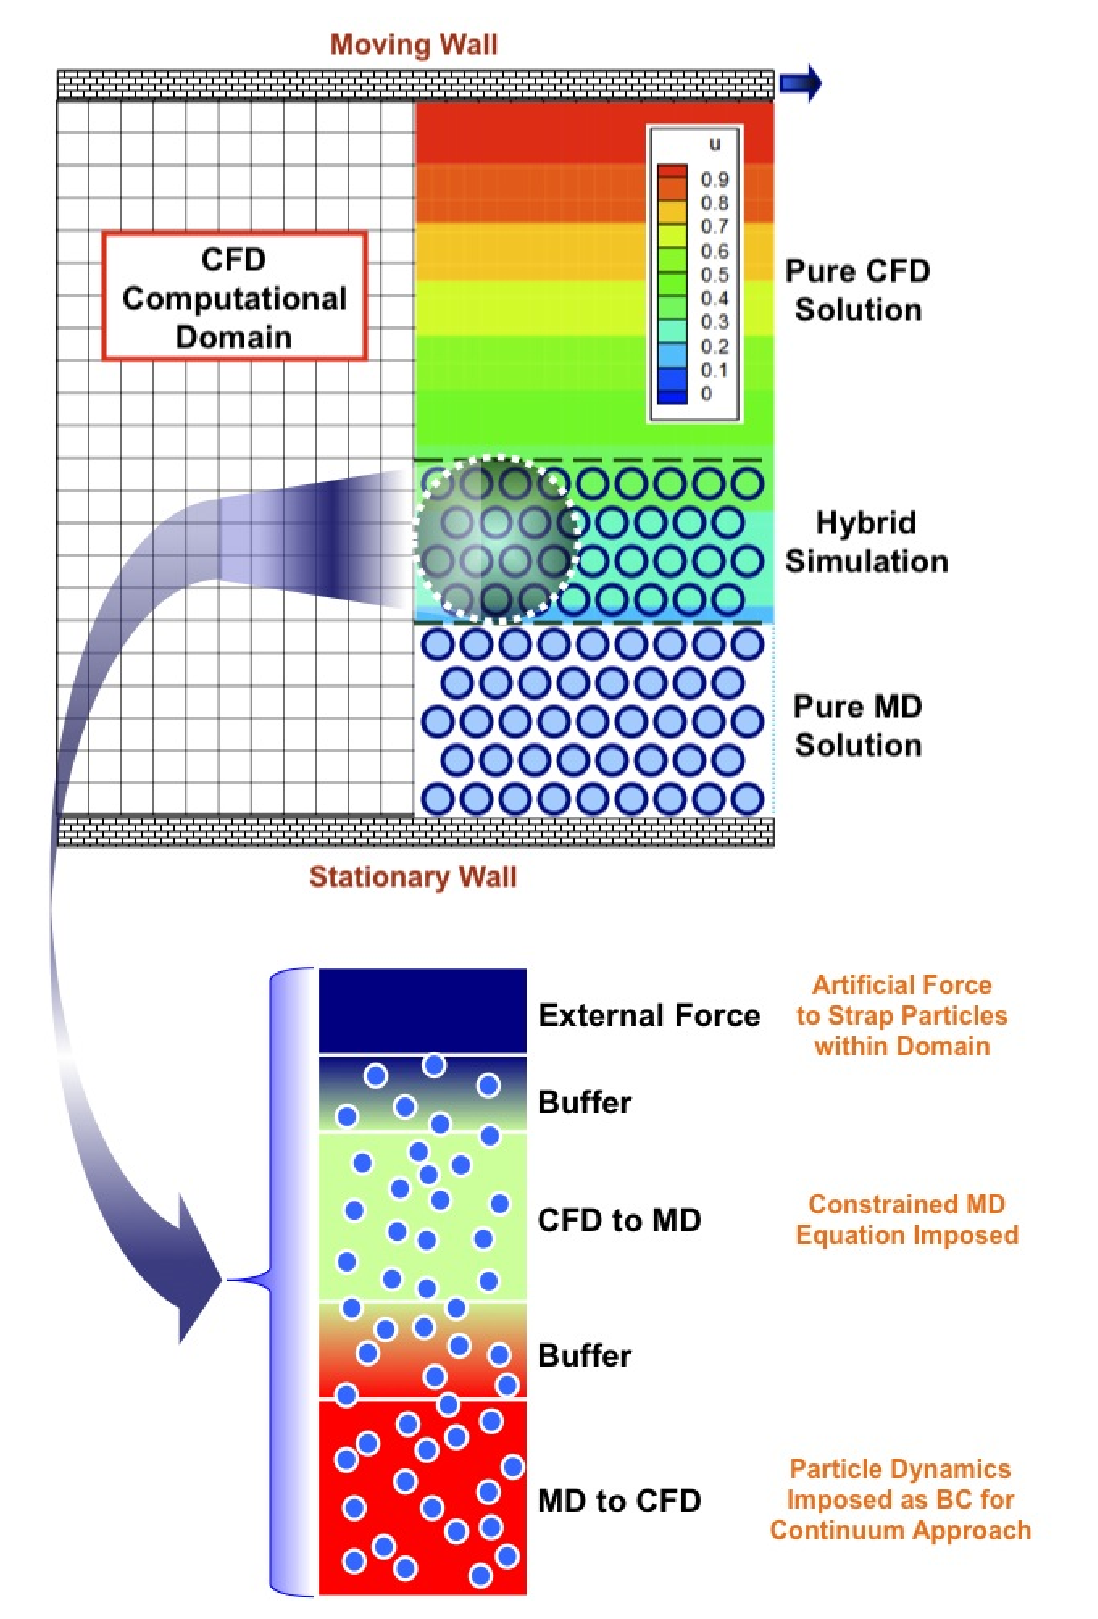
\includegraphics[scale=0.45]{fig1.eps}
\caption{\small Schematic of CFD/MD Coupled Simulation of Channel Flow}
\label{Fig:Couette}
\end{figure}
%%%%% FIGURE %%%%%

CFD-MD coupled simulation requires the design and implementation of hybrid coupling schemes such as control of exchanged information and physical models of constrained dynamics, on the basis of reliable CFD and MD simulation toolkits. We have developed an in-house incompressible CFD~\cite{Lee} and and employed the in-house modified version of LAMMPS~\cite{LAMMPS} for MD.

The coupling algorithm is embedded in Fig.~\ref{Fig:Couette}, which also illustrates the communications between the constituents of the hybrid code. Usually, this simulation is conducted where molecular-level effects are dominant on some region of the domain, for example, a nano-structured or surface-modified micro-scale channel. MD simulation is conducted near the solid material boundary where the interaction between the solid material and the fluid is on the molecular level. The macroscopic features are governed by the continuum equations solved through the CFD solver. A hybrid region is positioned between these regions to let the two domains exchange information.

The essence of this coupled approach lies in how the hybrid region is constructed and how data are exchanged between the MD and CFD solutions. As illustrated in right hand side of Fig.~\ref{Fig:Couette}, the hybrid region minimally consists of five subzones. The CFD boundary grid region is positioned near the pure MD region,. Velocities of particles within this zone are averaged and imposed as CFD boundary conditions for the corresponding computational cells. The MD boundary zone is placed above the CFD boundary zone. Here, velocities from the CFD grid are imposed on the MD through dynamically constrained MD equations. The dynamic constraint is introduced as a source term to the particle equation of motion which is appropriate to ensure that a macroscopic velocity from CFD and an averaged particle velocity from MD will eventually be the same. Between these zones, a buffer layer exists to transition the differences between the MD boundary and CFD boundary zones without direct influence of one on the other. If this zone is too narrow, particles in the CFD boundary zone become more directly influenced by particles in the constrained MD zone, allowing the CFD information to be passed through constrained dynamics directly back to the CFD solution. The truncated and shifted Lennard-Jones potential is implemented for evaluation of the intermolecular force during MD simulation.

The simulation procedure and the design of a problem domain is as follows: A computational domain is constructed using a CFD mesh generator and it is roughly split to three regions of pure MD, overlap and pure CFD. Then, the overlap region is split again to contain the five layers mentioned above. This geometric information is transferred to CFD and MD codes as input parameters, to define their computational domains. In our initial approach during the simulation, the CFD code stores flow properties within the constrained MD region in the form of a data file and reads a data file from the MD solution as its boundary condition. This is done for each iteration. The MD code also stores flow property data on CFD ghost cells and gets continuum property data for the constrained region. The difference is that, the MD code needs to average particle velocities inside prescribed CFD ghost zones over time as the time scale of MD processes is far less than that of the continuum CFD-resolved processes.

Another considerable issue in CFD-MD coupled simulation is execution and performance of using HPC resources, (e.g., problems caused by both simulation toolkits need to run concurrently on conventional queuing system and different size of two jobs require frequent communication during the simulation) which is referred to previous section. In order to avoid its computational complexity and give more efficiency, SAGA-based framework is employed not only solving the problems of coupled simulation, but also achieving dynamic load-balancing to reduce latency on the information exchange stage.


%\Nkimnote{ }
%-------------------------------------------------------------------------
\section{SAGA and Its Abstraction for Large-scale Computation}

\subsection{SAGA}

The Simple API for Grid Applications (SAGA) is an API standardization effort within the Open Grid Forum (OGF)~\cite{ogf_web}, an international standards development body concerned primarily with standards for distributed computing.  SAGA provides a simple, POSIX-style API to the most common Grid functions at a sufficiently high-level of abstraction so as to be %able to be
independent of the diverse and dynamic Grid environments. The SAGA specification defines interfaces for the most common Grid-programming functions grouped as a set of functional packages (Fig.~\ref{Fig:SAGA1}). Some key packages are:

\begin{figure}[!ht]
 \begin{center}
     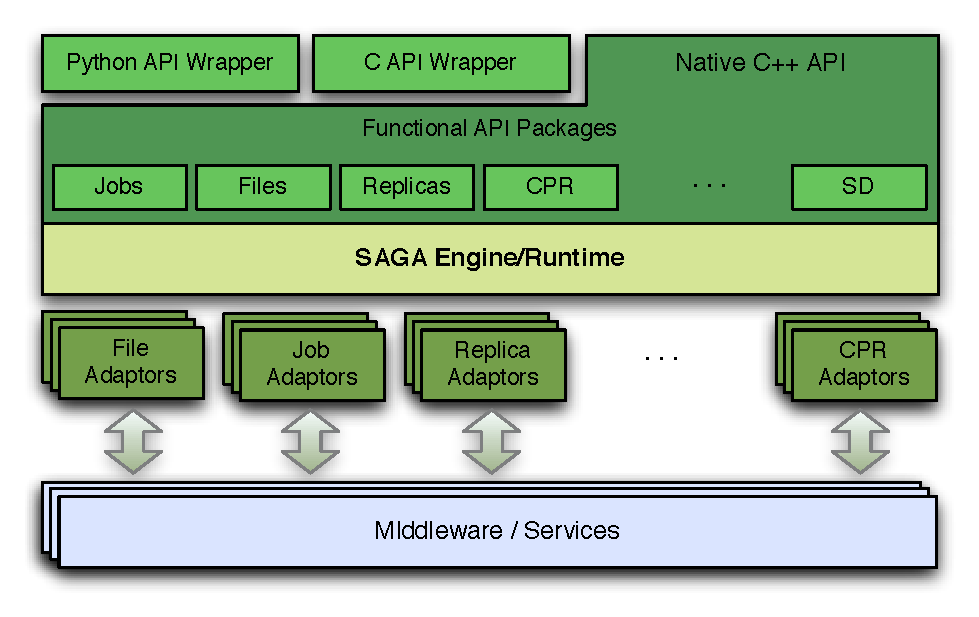
\includegraphics[width=0.40\textwidth]{stci_saga_figures-1.pdf}
 \end{center}
\caption{\small Layered schematic of the different components
  of the SAGA landscape. At the topmost level is the simple integrated API which provides the basic functionality for distributed computing. Our BigJob abstraction was built upon this SAGA layer using Python API wrapper} \label{sagalayer}
\end{figure}

%\begin{itemize}\addtolength{\itemsep}{-0.8\baselineskip}


\begin{itemize}
\item File package - provides methods for accessing local and remote
 filesystems, browsing directories, moving, copying, and deleting
 files, setting access permissions, as well as zero-copy reading and
 writing
\item Job package - provides methods for describing, submitting,
 monitoring, and controlling local and remote jobs. Many parts of
 this package were derived from the largely adopted
 DRMAA % ~\cite{drmaa_url}
 specification.
\item Stream package - provides methods for authenticated local and
 remote socket connections with hooks to support authorization and
 encryption schemes.
\item Other Packages, such as the RPC (remote procedure call) and Replica
 package
\end{itemize}


%\skonote{Introduction of PilotJob and BigJob (1 or 2 paragraphs) : What is PilotJob, BigJob / what have been done so far and how effective it was when using BigJob}



%\skonote{Joohyun, can you check this paragraph and improve it? In this paragraph, I was going to talk about 'Structure and Simulation Flow of BigJob Abstraction for Coupled Simulation'.}


Fig.~\ref{Fig:BigJob_Structure} shows the structure of BigJob and its operation flow. When a BigJob is submitted to the remote resource, the application manager monitors the status of this pilot-job through the advert service. When resources are allocated to the BigJob, the application manager divides obtained resources to its sub-jobs and a coupled simultion starts under the control of a multi-physics agent in the remote resource. Advert service keeps on getting the status of a pilot-job from the queueing system and the status of sub-jobs from multi-physics agent, also delivering these information to the application manager by a push-pull mechanism. The application manager watches the status of sub-jobs and decides the next event when the coupled simulation is finished. When one default BigJob is launched, subtasks keeps running until final solution is achieved and the manager quits the pilot-job at that time. In cases multiple BigJobs are submitted for the same simulation or a load balancing function is included, sub-jobs experience several restarts from their checkpoinitng data, reflecting changed processor allocation to each application. In former case, resource allocation to each sub-job follows a pre-defined map according to the number of BigJobs allotted to this simulation: In latter case, resource allocation to each sub-job becomes dynamic according to its performance, to be discussed in the next section.

%%%%% FIGURE %%%%%
\begin{figure}
\centering
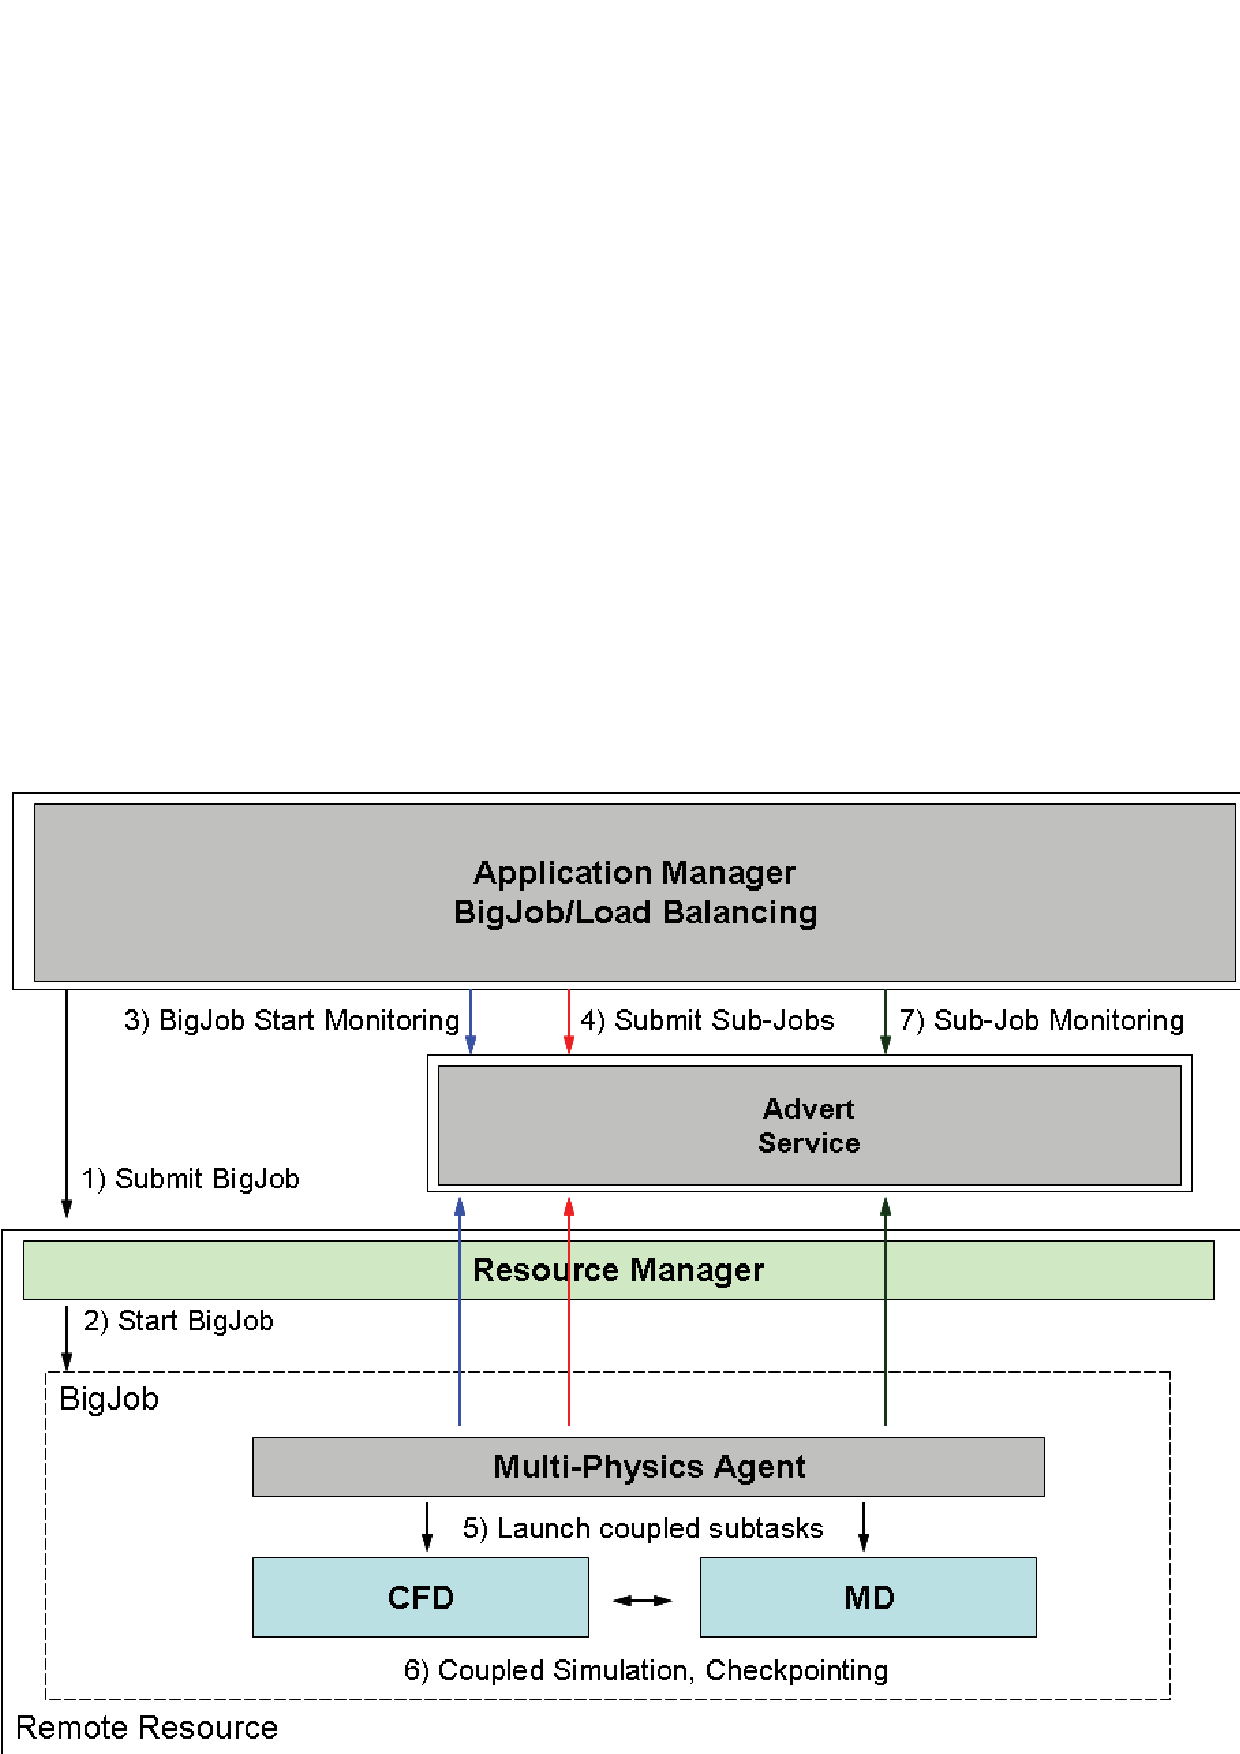
\includegraphics[scale=0.40]{Structure_of_BigJob}
\caption{\small Structure of BigJob and Its Operation Flow. Application manager carries out primarily job management including BigJob and sub-job submission, their status monitoring functions.  We implement a load balancing module, and migration service based on job information. Application agent system resides on each HPC resource and conducts job information gathering as well as communication with application manager via the advert service }
\label{Fig:BigJob_Structure}
\end{figure}
%%%%% FIGURE %%%%%



%-------------------------------------------------------------------------
\section{Load Balancing for Performance Enhancement of Coupled Multi-physical Simulation}


SAGA and its pilot-job framework (BigJob) enable coupled, yet distinct simulations to be
% by resolving the concurrency problem when coupled application codes are individually
submitted to queueing system.  This is done by submitting one container job, and re-distributing its processors to each task.  Also, total execution time can further be reduced by assigning more BigJobs and dynamically reallocating resources to each sub-task with increased number of processors.
However, the flexibility to re-distribute resources (processors) to the individual task, does
not imply efficient utilization. This is the responsibility of a load-balancer (LB)
We will discuss the implementation and algorithm of this LB; it is important
to mention that the LB functions in the context of the SAGA-BigJob framework.
% As the current simulation requires frequent data exchange between CFD and MD during the simulation, it is likely to increase communication cost (strictly, waiting time for communication in one application) if their loads are not well balanced, which is quite different from former BigJob application~\cite{Jha:2009} where data exchange takes place when sub-tasks stopped temporarily.

% Meanwhile, checking sub-tasks' performances and controlling their operation for load balancing runs counter to SAGA's philosophy of "using services without changing the application source". Thus, help from application side is necessary to employ a load balancing function on a BigJob.

Each applications load is determined by its elapsed time to run the evolution loop. Here, time for initialization or inter-domain data exchange are excluded from the counting, because they are one-time event or irrelevant to application's performance. As the result of load balancing is reflected in the next launch of simulation codes, applications should be able to restart from their checkpointing data. Also, they should be equipped with generalized domain partitioning routine to run simulation with any number of processors, without harming their parallel efficiency a lot.  If above conditions are satisfied, BigJob application manager,
can be interfaced with the LB to implement the dynamic resource allocation between tasks.
% load balancing between subtasks before applications restart from the previous state.
The idea of current load balancing algorithm is to assign more processors to a sub-task with more runtime until two codes show the same runtime. We have adopted some assumptions to simplify load balancing procedure and apply the algorithm without considering applications' characteristics and indivual code's scalability. Assumptions are, (1) Each application code follows the ideal parallel efficiency.
(2) All processors in one node is assigned to one sub-job.

%\begin{tabular}{|l|}
%\hline

%Let computation time of two applications by $t_CFD$ and $t_MD$, processors to each domain by $PE_CFD$ and $PE_MD$, respectively.
%Total workload $W_TOT$ is going to be \\

%\begin{equation}
%\begin{center}
%W_{TOT} = W_{CFD} + W_{MD} = PE_{CFD} \ times t_{CFD} + PE_{MD} \ times t_{MD}
%= PE_{TOT} \times t_{TOT}
%\end{center}
%\end{equation}

Let the computation time of two applications as $t_{CFD}$ and $t_{MD}$, processors to each domain as $PE_{CFD}$ and $PE_{MD}$, respectively. Based on assumption (1), workload on each application remains the same after the reallocation of resources,
\begin{eqnarray}
%\begin{center}
W_{CFD} &=& PE_{CFD} \times t_{CFD} = PE_{CFD}' \times t_{CFD}', \nonumber \\
W_{MD} &=& PE_{MD} \times t_{MD} = PE_{MD}' \times t_{MD}'
%$t_{CFD} = \frac {PE_{CFD} \times t_{CFD}} {PE_{CFD}} , ~~ t_{MD} = \frac {PE_{MD} \times t_{MD}} {PE_{MD}}$
%\end{center}
\label{eq:SimTime_EachTask}
\end{eqnarray}
Still, total number of processor remains the same:
\begin{equation}
%\begin{center}
PE_{TOT} = PE_{CFD} + PE_{MD} = PE_{CFD}' + PE_{MD}'
%\end{center}
\label{eq:PECondition}
\end{equation}
Our objective is to reduce the computation time of an over-loaded subtask until two simulations show the same computation time, $t_{CFD}' = t_{MD}'$. Then, Equation~\ref{eq:SimTime_EachTask} and Equation~\ref{eq:PECondition} concludes the optimal processors for one subtask would be
\begin{eqnarray}
%\begin{center}
PE_{CFD}' & = & \frac {W_{CFD}} {(W_{CFD} + W_{MD})} \times PE_{TOT}
%\end{center}
\end{eqnarray}
The other sub-job will follow the similar expression.
The optimal processor distribution from above equation will return a float value. Also, considerting the second assumption, which is the policy of many supercomputing center, the above distribution needs to be asymptotic. If CPU cores in one node is $N_{UNIT}$,
%$N_{UNIT} \times S < PE_{CFD}' < N_{UNIT} \times (S+1)$, we can choose the optimal condition by comparing $MAX(t_{CFD}',t_{MD}')$ between upper and lower bound of processor allocation.
optimal condition can be gained by finding $S = int(PE_{CFD}' / N_{UNIT})$ and comparing $MAX(t_{CFD}',t_{MD}')$ in cases CFD task is allocated with $N_{UNIT} \times S$ or $N_{UNIT} \times (S+1)$.


%\hline
%\end{tabular}

%The control-flow within the BigJob Application-Manager when supporting a LB modules is shown in Fig.~\ref{Fig:BigJob_LB}. When one simulation loop is finished, the performance data of each subtask is sent to the load balancing module and it computes optimal resource distribution. Sub-job launcher restarts coupled application codes from their checkpointing data, according to the result of load balancing function. This process iterates until coupled simulation finalizes and processor allocation moves to the optimal condition during this process.

%%%%% FIGURE %%%%%
%\begin{figure}
%\centering
%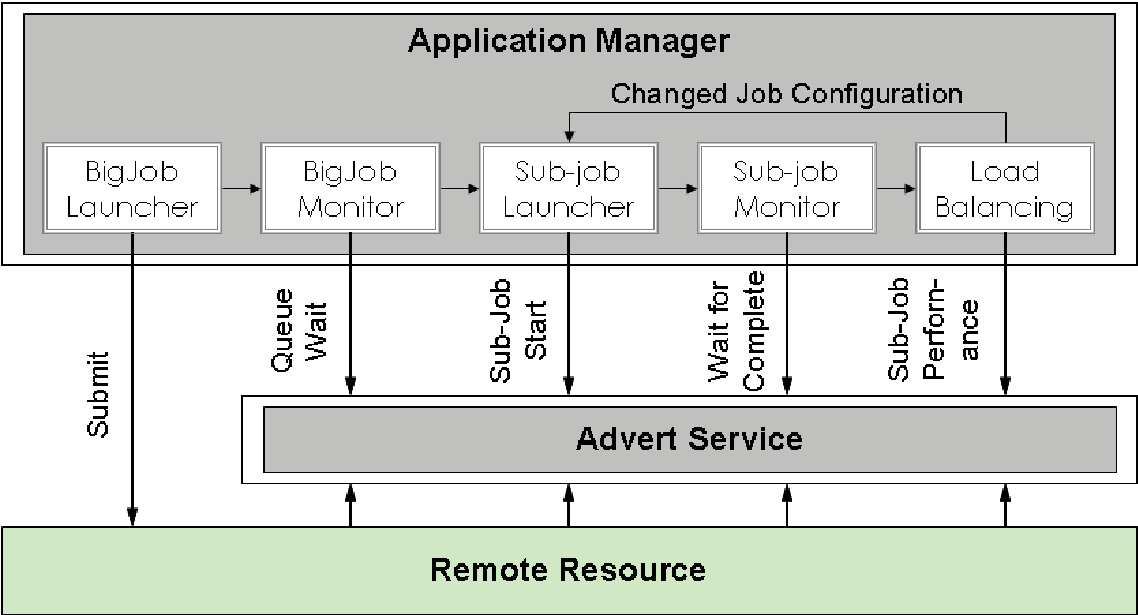
\includegraphics[scale=0.40]{BigJob_with_Load_Balance}
%\caption{\small Operation Flow of a BigJob with Load Balancing Function}
%\label{Fig:BigJob_LB}
%\end{figure}
%%%%% FIGURE %%%%%



%-------------------------------------------------------------------------
\section{Three Use Cases of Hybrid CFD/MD Simulation using SAGA and SAGA-based Framework}

In Section 2, we have argued the challenges of running a coupled multi-physical simulation on a conventional queueing system as (i) Hardness to start multiple applications concurrently; (ii) Unability to balance the load among domains, and (iii) Fixed number of allocated resources throughout the simulation.  To resolve the co-scheduling and load-imbalance issues, and with the ultimate aim of reducing the time to solution, we have used the BigJob abstraction with load balancing module to the coupled simulation. % With the ultimate aim of reducing the total simulation time, we investigate acquiring idle resources during the simulation, by launching multiple BigJobs for one coupled simulation.
Three different real scenarios arise. In the first, a single BigJob is utilized to run the coupled-simulations, first without, and then with the LB redistributing resources based upon their individual performance. One component maybe relieved of its resources for the greater good. In the second Use Case, In the second case, two BigJobs are started together, but often one BigJob starts before the other; to increase efficiency both coupled simulations start with whatever resources are available as part of the first (to run) BigJob. When the other BigJob becomes active, there is a dynamic redistribution of tasks, such that
the larger of the two simulations is assigned the bigger BigJob. The variant of the above when
the two BigJobs are on different machines forms Use Case 3. In the remainder of this section we discuss
the details of these three different Use Cases.

% We compare the performance as measured by TTS using the benchmark case to be the situation when we do not have the ability to utilize the BigJob concept and thus each simulation interacts with the queueing system differently, and thereby each must be in an Active state before both can start running.

\jhanote{please be sure to use co-scheduling where appropriate and not concurrency}

\subsection{One BigJob with Load Balancing}
Fig.~\ref{Fig:OneBJ_Flow} shows the flow of a coupled simulation with the conventional job submission and through one BigJob. In a conventional way, individual tasks with resource requirements of $PE_{CFD}$ and $PE_{MD}$, respectively, are independently submitted to the conventional queueing system and job scheduler recognizes these coupled tasks as two distinct jobs. Thus, they are going to start at a different time, except when enough resources are idling. In this case, total simulation time ($t_{f0}-t_{0}$) is the sum of waiting time on the queue (the time no simulation is running, $t_1-t_0$), inactive mode (when one of tasks is waiting for another simulation's data, $t_2-t_1$) and active mode ($t_{f0}-t_2$).
If these tasks are submitted as a pilot job with the size of $PE_{CFD}+PE{MD}$, the inactive mode disappears as a BigJob manager will distribute allocated resources to subtasks. In this case, total simulation time changes to be the sum of waiting on the queue ($t_{1}'-t_{0}$) and simulation runtime ($t_{f1}=t_{1}'$). If resource distribution to subtasks is identical to the conventional job submission, total runtime will remain the same. It means that a user can save his/her account by the multiplication of first processor allocation and inactive time ($PE_{CFD} \times t_2-t_1$ in this example). However, eliminating inactive mode does not guarantee total simulation time is reduced, because waiting to get one allocation with $PE_{CFD}+PE_{MD}$ size can take more than getting two allocations with smaller chunks. The same situation can happen to the load-balanced case with one BigJob, which satisfies the reduction of total runtime compared to other examples.

%%%%% FIGURE %%%%%
\begin{figure}
\centering
\includegraphics[scale=0.40]{Simulation_Time_of_One_BigJob.eps}
\caption{\small Comparison of work flows between conventional job submission scenario and our scenario implemented with one bigjob submission.  The last column illustrates the load balancing function with one bigjob scenario}
\label{Fig:OneBJ_Flow}
\end{figure}
%%%%% FIGURE %%%%%



Table~\ref{table:oneBJ_Test} shows elspsed time on running above testcases: conventional job submission, one default BigJob launch and one BigJob with load balancing. These tests were conducted on supercomputing resources in LONI (Louisiana Optical Network Initiative)~\cite{LONI_web} and tested resources of eric, oliver and louie have the same specification with 4 processors in each node. A coupled simulation has been conducted by using 32 processors with two dirrenent processor allocations to subtasks. Application codes experience four restarting from their checkpointing data in load balancing test, while simulation keeps running until it completes in baseline and default BigJob tests.
From the first test of assigning 8 processors to CFD task and others to MD, conventional job submission and one default BigJob launch show nearly the same active runtime, as we have already expected. Comparing these two tasks, main difference lies in the existence of idling time on conventional job submission, which is denoted as 'inactive mode' in the table, when one of subtasks were allowed to start faster than BigJob submission but had to idle waiting for its counterpart. As a result, conventional testsuite starts later than one BigJob application, let alone the wasting of computing time on idling. Nevertheless, one BigJob submission does not guarantee faster start if we refer to the result of load-balanced BigJob submission, which experienced far longer waiting on the queue. For the worse, a load-balanced BigJob showed longer runtime than other tests, because additional cost on running a load balancing function and trying checkpointing and restarting subtasks is not compensated by the performance improvement in this well-defined resource assignment.
On the other hand, load balancing becomes effective at initially imbalanced condition. When same number of processors are assigned to each subtask, load balancing function leads the resource allocation to the best condition after the first simulation loop and 8 processors from CFD task are moved to MD simulation from the next start, which is the same as former resource allocation. Thus, the performance in load balanced case becomes identical to above tests from the second start and total runtime shows far better result than other imbalanced cases. Still, load balaced case experiences longest total simulation time because of long waiting on the queue, which is case-specific.



% Elapsement for a CFD/MD Coupled Simulation by using Conventional Queueing System and a BigJob Abstraction. Above table shows total simulation time when 8 processors are allocated to CFD and 24 processors on MD task, which is initially well-balanced allocation: below one represents another test with 16 processors allocated to each task, an imbalanced simulation. Values in table shows averaged time in seconds, values within a parenthesis are standard deviation of time elapsed; the average is taken over 5 distinct
% experiments. \newline }


\begin{table}[!h]
\begin{center}
\label{table:oneBJ_Test}
\caption{\small Results for performance data using BigJob with and without LB. The Baseline Simulation represents the case when BigJob is not used; in this case, the time to start is dominated by the Inactive Mode of the longer waiting task. The use of BigJob resolves, this as can be seen by the reduced inactive mode time in columns
3 and 4. The starting configuration assigns resources equally between CFD-MD -- 16px each. However, after a few iterations of the LB the configuration is 8-24. It is with this configuration that the performance is better with LB, than without the LB 1370 $\pm 98$ vs 1641 $\pm$ 162. The starting configuration of the second set (8-24) is a ``balanced configuration'' which is why there is no performance gains on using the LB. Values in table shows averaged time in seconds, values within a parenthesis are standard deviation of time elapsed; the average is taken over 5 distinct experiments}
% experiments. }
%\label{table:systems}
\begin{tabular}{ c|| c | c | c }
\hline
16-16 & Baseline Simulation & BigJob (no LB) & BigJob (LB) \\
\hline
\hline
Waiting on & 3000 & 10834 & 15201  \\
the Queue & (4136) & (4593) & (10968) \\
\hline
Inactive & 10300 & 4 & 4 \\
Mode & (15327) & (0) & (0) \\
\hline
Active & 1672 & 1641 & 1370 \\
Runtime & (246) & (162) & (98) \\
\hline
Total & 14973 & 12480 & 16577 \\
Time & (19213) & (4430) & (11004) \\
\hline
\end{tabular}
\begin{tabular}{ c|| c | c | c }
\hline
8-24 & Baseline Simulation & BigJob (no LB) & BigJob (LB) \\
\hline
\hline
Waiting on & 1900 & 3372 & 10344  \\
the Queue & (1873) & (6450) & (6767) \\
\hline
Inactive & 5486 & 4 & 4 \\
Mode & (10318) & (0) & (0) \\
\hline
Active & 1171 & 1169 & 1280 \\
Runtime & (175) & (72) & (81) \\
\hline
Total & 8557 & 4545 & 11629 \\
Time & (11882) & (6457) & (6720) \\
\hline
\end{tabular}
\end{center}
\end{table}


A number of performance tests with different initial job allocation have been conducted and graphs in Fig.~\ref{fig:LB_Graph} show the result. From the first test when 32 processors are used, load balancing function detects the ratio of 8 and 24 between CFD and MD tasks are optimal and converges to this ratio at the next restart, except one case when CFD solution experiences unexpected overload initially. Though CFD simulation still shows far less runtime compared to MD work, load balancing function judges this configuration is optimal, because CFD simulation time is estimated to be longer than current MD time if processors allotted to CFD reduces to 4. Remember that processor allocation changes by the number of processors in each node. Also, the above decision is verified by the next load balacing test where the ratio of 4 and 20 between CFD and MD tasks are ideal. In this simulation, CFD runtime with 4 processors is longer than 200 seconds, which is longer than MD simulation time with 24 processors. This means that total runtime would be increased if processor distribution changes from 8 and 24 to 4 and 28. Focusing on the load balancing test with 24 processors again, CFD and MD tasks show nearly the same simulation time after converged processor allocation is gained. Also, load balancing function indicates the optimal condition after the first sub-job running, except one variation when initial CFD task was running with doubled CPUs than MD task. Even in this case, load balancing function traces the optimal load allocation during the iteration and this demonstrates the stability of current load balancing function.

%%%%% FIGURE %%%%%
\begin{figure}
\centering
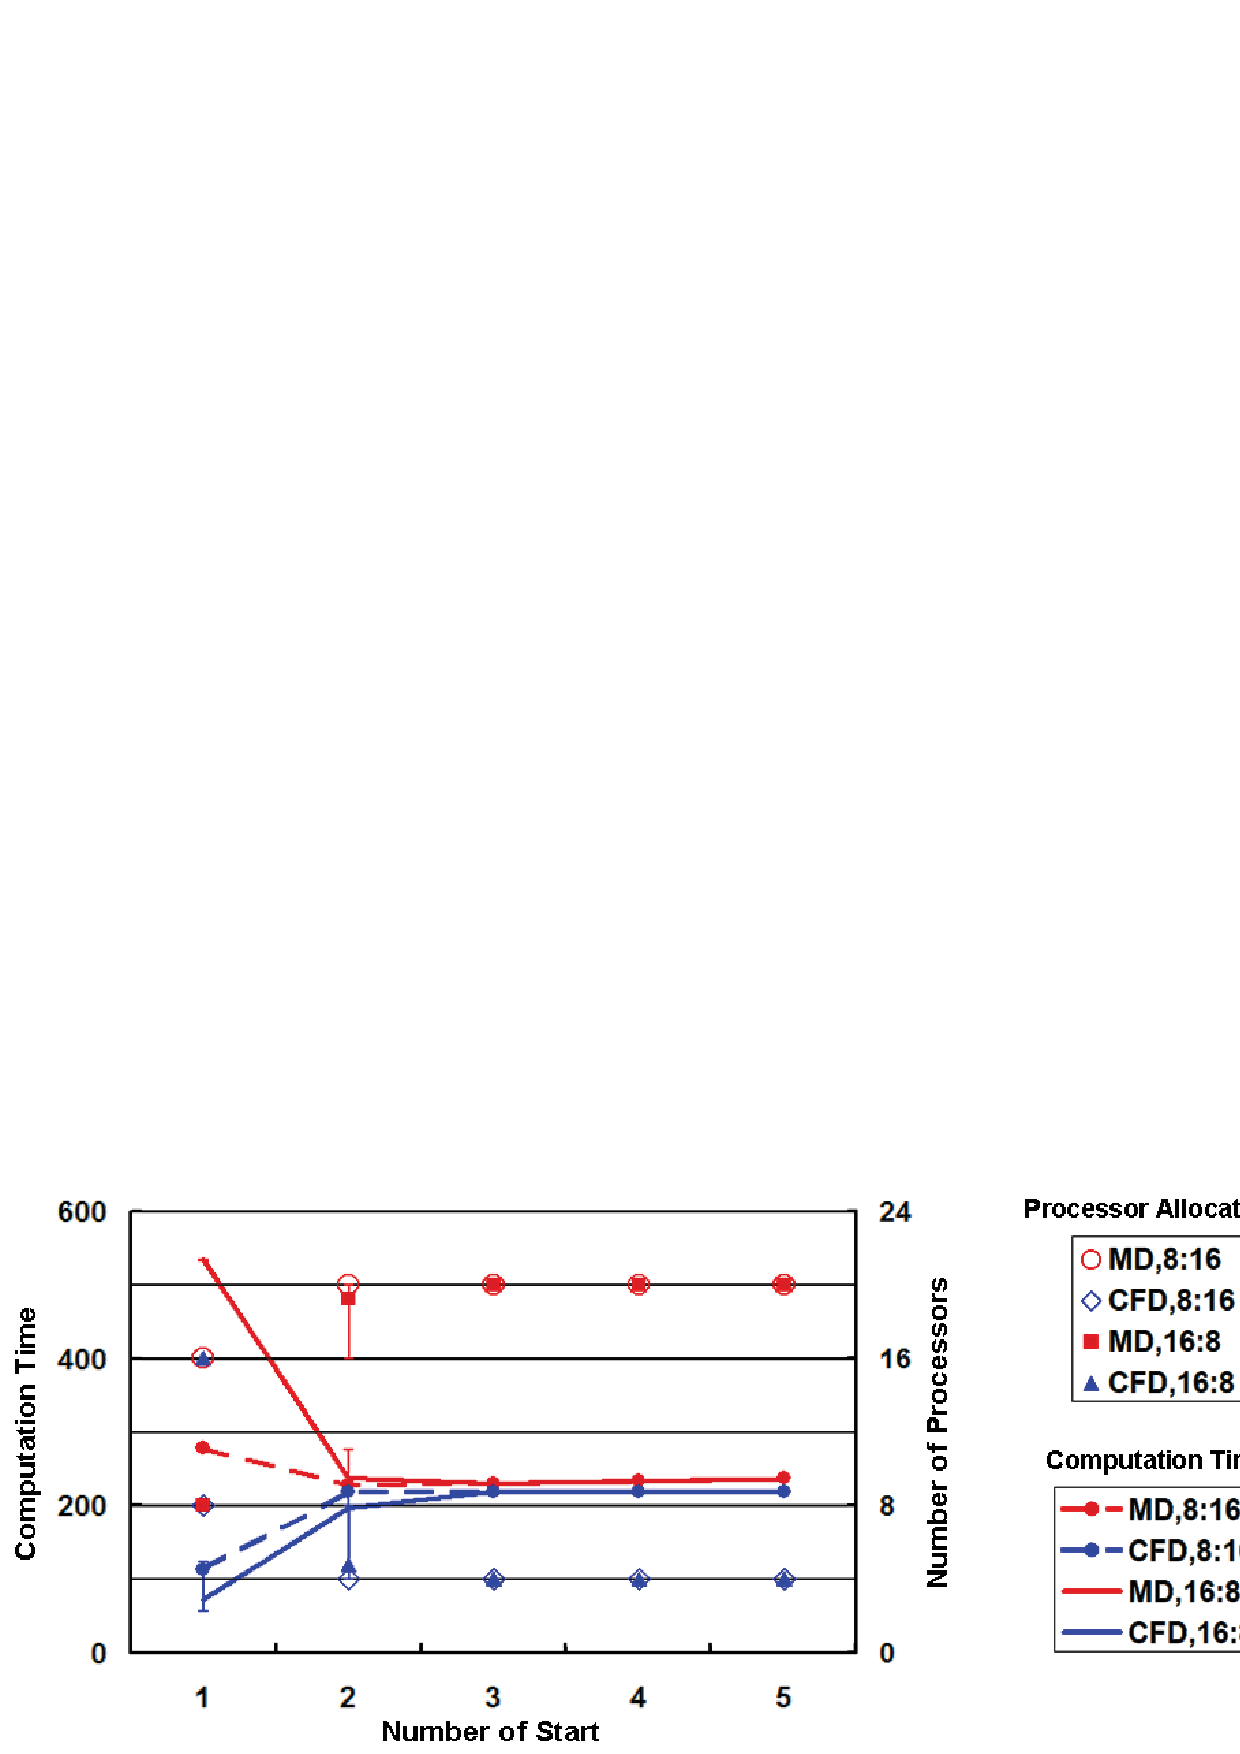
\includegraphics[scale=0.25]{LB_Graph}
\caption{\small Convergence of a Load Balancing Function and Runtime of Suntasks. Above graphs show load balancing result when 32 processors are assigned initially. Latter graphs represent the history of load balancing when 24 processors are allocated.}
\label{fig:LB_Graph}
\end{figure}
%%%%% FIGURE %%%%%

Though the above results show the large performance gain by employing a load balancing algorithm, some limitations are also observed. First, as the function only refers to the computation cost at given processor distribution and moves to the optimal condition iteratively, it takes time to achieve a converged resource allocation if initial processor allocation starts from other extreme. Second and furthermore, the alogrithm itself should be refined to distinguish the computational cost from inter-processor communication within one application code and control both factors. Also, the load balancing module needs to be expanded to cover multiple BigJob allocations for one coupled simulation, when running a subtask across BigJobs becomes possible.


\subsection{Two BigJobs from a Single Site or Multiple Sites}


As illustrated in Figure~\ref{Fig:TwoBigJobs}, runtime environment for coupled multi-physics simulations would benefit from dynamic resource availability exploited by BigJob implementation. In brief, it is possible to assign more CPUs for a slowing application when another BigJob becomes available. Compared with one BigJob allocation for a coupled simulation in Figure~\ref{Fig:One_BigJob_Run}, two smaller BigJob submissions with sizes of CFD and MD will enable faster start of coupled subtasks. Also, when next BigJob is also allocated to this coupled simulation, total job size will be the same as one BigJob submission. In a word, resource allocation and simulation flow is identical to the conventional job submission, but inactive idling in a conventional case disappears as a BigJob framework starts coupled subtasks with smaller number of processors when first job is allocated. So, submitting two BigJobs guarantees the reduction of total simulation time compared to conventional job submission, if all conditions are identical. If this two BigJob submission is applied on multiple sites, it is more likely to get two allocations faster than requesting two jobs in the same site. However, faster launch of two BigJobs does not guaranteed save of total simulation time, because time for data exchange between applications will also increase if distributed resources cooperate.


%%%%% FIGURE %%%%%
\begin{figure}
\centering
\includegraphics[scale=0.40]{Simulation_Time_of_Two_BigJobs.eps}
\caption{\small Schematic of work flows for a job submission with two bigjobs at the Same Site and Multiple Sites}
\label{Fig:TwoBigJobs}
\end{figure}
%%%%% FIGURE %%%%%


In Table~\ref{table:TwoBigJobs}, test measurements for performance gains are summarized. The scenario for this testing is simple for clarifying benefits.  Initially, two bigjobs are submitted to one HPC resource or two HPCs.  Once the first bigjob becomes available, two applications are submitted as two subtasks with pre-defined cpus to the bigjob, and then when another bigjob becomes available later, two subtasks for each application is reconfigured by assigning the entire cpus of a bigjob to one application.  Table  ~\ref{table:TwoBigJobs} shows performance gains with such a scenario in terms of MD run time.  In this simple scenario, other complicated aspects such as file transfer, in particular between two distributed resources are not considered but in the future study, the overall performance will be optimized by considering them.

% Performance gains with two bigjobs. Performance is measured with CPU times consumed by MD, since test cases we used always require longer cpu times for MD than those of CFD.  Performance gains with additionally available bigjob can be seen by comparing MD CPU times with those obtained with the initial bigjob.  Measurements were carried out with LONI cluster systems.  louie and poseidon are dell cluster systems having 128 nodes with 4 cores in a node. \jhanote{add bigjob size --- which 8 and 16} Test 1 and 2 correspond to Use Case 2; Test 3 and 4 correspond to Use Case 3 \newline }

\begin{table}[!h]
\begin{center}
 \caption{\small
Performance measures for Use Cases 2 and 3. We take the time of the MD simulation as a measure of peformance.
For Test 1 and 2, we compare the time taken (for the MD simulation) before and after the availabilty of
the second BigJob. As can be seen, the time to solution is significantly lower. This is now because
the entire second BigJob is available to the MD simulation.
For Test 3 and 4, the second BigJob (i.e the one to start later) is launched on a different machine
from the first BigJob. For similar reasons to Test 1\&2, the time to solution is lower when the
second BigJob starts. This situation will win over the single BigJob scenario, even inspite of transfer/set-up times. For Test 1-3, the size of the first BigJob is 8px, whilst the size of the second (later avialable) BigJob is 16px. For Test the first BigJob is 16px and the second BigJob is 32px.}
\label{table:TwoBigJobs}
\begin{tabular}{ c| c c c c }
\hline
& Test 1   & Test 2 & Test 3   & Test 4 \\
\hline
number of sites & 1 & 1 & 2 & 2  \\
site names & P & L  & L + P & L + P \\
\hline
(one bigjob available) & & & & \\
number of cpus assigned & 4 & 4 & 4 & 8 \\
MD CPU time  (sec) & 1037.2 & 1045.2 & 1049.0 & 534.2  \\
\hline
(two bigjobs available) & & & & \\
number of cpus assigned & 16 & 16 & 16 & 32 \\

MD CPU time  (sec) & 277.21 & 277.63  & 276.8 & 150.4  \\

\hline
\end{tabular}
\end{center}
\end{table}



\skonote{Joohyun and Abhinav: Simulation results will come here}

In summary, use of a BigJob will eliminate idling operation of a subtask, which waits for another application to start running. Also, employing a load balancing function will let coupled codes use allocated resources more efficiently. Furthermore, using two BigJobs promotes the reduction of total simulation time, compared to conventional job submission. Meanwhile, launch of two BigJobs does not intend to use resources more efficiently than conventional job allocation, but intend to save total simulation time more than one BigJob test case, by utilizing more available resources. Remember that having multiple BigJob allocations is to increase the computing power for a specific simulation, not to use optimally within given circumstances.


%-------------------------------------------------------------------------
\section{BigJob: A General Purpose Pilot-Job}

%The concept of a Pilot-Job has been advanced by the Condor project, wherein the Pilot-Job concept is referred to as a Glide-in...  Here we will discucss (i) how SAGA-BigJob has been used in conjunction with Condor-Glide-in whereby SAGA-BigJob was used on the TeraGrid (Ranger) and the Glide-in was running on the Purdue Condor Cluster.

With minor modifications to the BigJob asbtraction layer, we are able to submit jobs to condor pools in addition to TeraGrid resources. To that end we use Condor's native pilot-job (Glide-In) for Condor resources, through the SAGA Condor adaptor. This allows us to concurrently make use of high performance resources on the TeraGrid and high-throughput resources such as the condor pools at Purdue and LONI. Having the capability to run pilot jobs on both types of resources through a unifed abstract interface with varying underlying mechanisms presents new opportunities for Grid interoperability research and hybrid coupled simulations.

To demonstrate interoperability, we started a BigJob (the core supercomputer of LONI) to which we submitted a molecular dynamics simulation. Once the molecular dynamics simulation has finished successfully, it's coupled CFD simulation is submitted to the Condor Pool at Purdue through the Condor Glide-In. The total time spent running on QueenBee was 5328 seconds, and the total run time on the Condor poll was 1015 seconds for a reduced size problem. The reduction in problem size was necessary due to the lack of a working MPI Condor universe on an accessible resource.


\section{Conclusions}
% We present data indicating performance advantage at almost every stage of progressive sophistication.
% performance figures show, there is significant improvement in the time-to-solution

Increasing accessibility to High Performance Computing and advances in software development utilizing parallelism implemented in different granularity are, perhaps, two critical components for recent numerous successful outcomes with large scale scientific calculations in various domains. Nonetheless, it is a non-trivial task
to develop and deploy approaches that support effective runtime execution
on both distributed systems (at scale) and on monolithic high-end systems.
Specifically, in this work, we report on progress in implementing efficient runtime solutions
that faciliate coupled multi-physics application (comprising MD and CFD).
%to utilize as two coupled standalone applications.  
In addition to desigining for extensibility and scalability, overcoming the need for an external co-scheduler and supporting dynamic resource allocation mechanism so as to support load-balancing, were two main goals motivating this work. Our development is built upon the BigJob framework enabled by the SAGA.
We began by performing coupled simulations as components negotiating with the scheduler independtly; we observed that in the absence of co-scheduling this approach is not very effective.  We performed experiments that first showed how the use of SAGA-based BigJob by providing a container-job, overcame the need for effective execution without co-scheduling. Interestingly BigJob also provided the ability to dynamically reassign resources relatively between the CFD and MD components, which is critical for most Load Balancing mechanisms.  Under the fundamental execution principle that it is better to start execution on whichever resource is avialable first, and dynamically adjust to a more optimal resource when it become available, our subsequent experiments involved two BigJobs, which although launched simultaenously did not begin execution simultaneously. However, in spite of the cost of re-assignment and even distributed placement to utilize the second BigJob, our experiments indicate that overall performance is better with a run-early dynamic execution model, than alternatives.

% integrate a targeted scientific application with a resource management system that is aware of the challenges arising from the distributed computing as well as the local scheduler implemented with the local resource management policy.  

% a novel development and our test runs demonstrated its potential for large scale scientific simulations benefiting scientific problems that are only tackled by a coupled hybrid MD-CFD calculation.
% The cycle of the development for core BigJob management system is significantly helped by using the SAGA with which the simple and consistent interface for managing HPC resources is easily achieved resulting the agile and flexible development.
% We tested our development for three cases and demonstrated its capability.  In addition, the use cases includes the usage of the Condor-glide-in as our BigJob framework is closely related.  In spite of simple nature of our test problems, already our development showed many promises for a successful large scale simulation.  Some of those are i) employment of load balancing mechanism ii) advantages from implementation of dynamic allocation in heterogeneous distributed computing resources iii) simple solution for the co-scheuling requirements for the coupled tasks.

\section*{Acknowledgement}
This work is part of the Cybertools (http://cybertools .loni.org) project and primarily funded by NSF/LEQSF (2007-10)-CyberRII-01. Important funding for SAGA has been provided by the UK EPSRC grant number GR/D0766171/1 (via OMII-UK).  This work has also been made possible thanks to computer resources provided by LONI.  We thank Andre Luckow for initial work on BigJob, Lukasz Lacinski for help with SAGA deployment (via HPCOPS NSF-OCI 0710874) and Joao Abecasis for his work on the SAGA Condor adaptors.

%-------------------------------------------------------------------------
\nocite{ex1,ex2}
%\bibliographystyle{latex8}
\bibliographystyle{IEEEtran}
\bibliography{saga_tg08}


\end{document}




%-------------------------------------------------------------------------
\section{Instructions}

Please read the following carefully.

%-------------------------------------------------------------------------
\subsection{Language}

All manuscripts must be in English.

%-------------------------------------------------------------------------
\subsection{Printing your paper}

Print your properly formatted text on high-quality, $8.5times 11$-inch
white printer paper. A4 paper is also acceptable, but please leave the
extra 0.5 inch (1.27 cm) at the BOTTOM of the page.

%-------------------------------------------------------------------------
\subsection{Margins and page numbering}

All printed material, including text, illustrations, and charts, must be
kept within a print area 6-7/8 inches (17.5 cm) wide by 8-7/8 inches
(22.54 cm) high. Do not write or print anything outside the print area.
Number your pages lightly, in pencil, on the upper right-hand corners of
the BACKS of the pages (for example, 1/10, 2/10, or 1 of 10, 2 of 10, and
so forth). Please do not write on the fronts of the pages, nor on the
lower halves of the backs of the pages.


%------------------------------------------------------------------------
\subsection{Formatting your paper}

All text must be in a two-column format. The total allowable width of
the text area is 6-7/8 inches (17.5 cm) wide by 8-7/8 inches (22.54 cm)
high. Columns are to be 3-1/4 inches (8.25 cm) wide, with a 5/16 inch
(0.8 cm) space between them. The main title (on the first page) should
begin 1.0 inch (2.54 cm) from the top edge of the page. The second and
following pages should begin 1.0 inch (2.54 cm) from the top edge. On
all pages, the bottom margin should be 1-1/8 inches (2.86 cm) from the
bottom edge of the page for $8.5 \times 11$-inch paper; for A4 paper,
approximately 1-5/8 inches (4.13 cm) from the bottom edge of the page.

%-------------------------------------------------------------------------
\subsection{Type-style and fonts}

Wherever Times is specified, Times Roman may also be used. If neither is
available on your word processor, please use the font closest in
appearance to Times that you have access to.

MAIN TITLE. Center the title 1-3/8 inches (3.49 cm) from the top edge of
the first page. The title should be in Times 14-point, boldface type.
Capitalize the first letter of nouns, pronouns, verbs, adjectives, and
adverbs; do not capitalize articles, coordinate conjunctions, or
prepositions (unless the title begins with such a word). Leave two blank
lines after the title.

AUTHOR NAME(s) and AFFILIATION(s) are to be centered beneath the title
and printed in Times 12-point, non-boldface type. This information is to
be followed by two blank lines.

The ABSTRACT and MAIN TEXT are to be in a two-column format.

MAIN TEXT. Type main text in 10-point Times, single-spaced. Do NOT use
double-spacing. All paragraphs should be indented 1 pica (approx. 1/6
inch or 0.422 cm). Make sure your text is fully justified---that is,
flush left and flush right. Please do not place any additional blank
lines between paragraphs. Figure and table captions should be 10-point
Helvetica boldface type as in
\begin{figure}[h]
  \caption{Example of caption.}
\end{figure}

\noindent Long captions should be set as in
\begin{figure}[h]
  \caption{Example of long caption requiring more than one line. It is
    not typed centered but aligned on both sides and indented with an
    additional margin on both sides of 1~pica.}
\end{figure}

\noindent Callouts should be 9-point Helvetica, non-boldface type.
Initially capitalize only the first word of section titles and first-,
second-, and third-order headings.

FIRST-ORDER HEADINGS. (For example, {\large \bf 1. Introduction})
should be Times 12-point boldface, initially capitalized, flush left,
with one blank line before, and one blank line after.

SECOND-ORDER HEADINGS. (For example, {\elvbf 1.1. Database elements})
should be Times 11-point boldface, initially capitalized, flush left,
with one blank line before, and one after. If you require a third-order
heading (we discourage it), use 10-point Times, boldface, initially
capitalized, flush left, preceded by one blank line, followed by a period
and your text on the same line.

%-------------------------------------------------------------------------
\subsection{Footnotes}

Please use footnotes sparingly%
\footnote
  {%
    Or, better still, try to avoid footnotes altogether.  To help your
    readers, avoid using footnotes altogether and include necessary
    peripheral observations in the text (within parentheses, if you
    prefer, as in this sentence).
  }
and place them at the bottom of the column on the page on which they are
referenced. Use Times 8-point type, single-spaced.


%-------------------------------------------------------------------------
\subsection{References}

List and number all bibliographical references in 9-point Times,
single-spaced, at the end of your paper. When referenced in the text,
enclose the citation number in square brackets, for example~\cite{ex1}.
Where appropriate, include the name(s) of editors of referenced books.

%-------------------------------------------------------------------------
\subsection{Illustrations, graphs, and photographs}

All graphics should be centered. Your artwork must be in place in the
article (preferably printed as part of the text rather than pasted up).
If you are using photographs and are able to have halftones made at a
print shop, use a 100- or 110-line screen. If you must use plain photos,
they must be pasted onto your manuscript. Use rubber cement to affix the
images in place. Black and white, clear, glossy-finish photos are
preferable to color. Supply the best quality photographs and
illustrations possible. Penciled lines and very fine lines do not
reproduce well. Remember, the quality of the book cannot be better than
the originals provided. Do NOT use tape on your pages!

%-------------------------------------------------------------------------
\subsection{Color}

The use of color on interior pages (that is, pages other
than the cover) is prohibitively expensive. We publish interior pages in
color only when it is specifically requested and budgeted for by the
conference organizers. DO NOT SUBMIT COLOR IMAGES IN YOUR
PAPERS UNLESS SPECIFICALLY INSTRUCTED TO DO SO.

%-------------------------------------------------------------------------
\subsection{Symbols}

If your word processor or typewriter cannot produce Greek letters,
mathematical symbols, or other graphical elements, please use
pressure-sensitive (self-adhesive) rub-on symbols or letters (available
in most stationery stores, art stores, or graphics shops).

%------------------------------------------------------------------------
\subsection{Copyright forms}

You must include your signed IEEE copyright release form when you submit
your finished paper. We MUST have this form before your paper can be
published in the proceedings.
>>>>>>> .r1604
>=======
=======>>>>>>> .r1615
